% RAVI (Reverse Action from Video): Learning Reverse Actions from Video -- JCSE (KIISE) regular paper draft.
% Main paper without appendices.
% Build: pdflatex RAVI_Main_2026; bibtex RAVI_Main_2026; pdflatex RAVI_Main_2026; pdflatex RAVI_Main_2026
\documentclass{jcse}

\usepackage{url}
\usepackage{amsmath}
\usepackage{amssymb}
\usepackage{graphicx}
\usepackage{booktabs}
\usepackage{multirow}
\usepackage{tikz}
\usetikzlibrary{arrows.meta,positioning,fit,calc}
\definecolor{actc}{HTML}{2A78D6}  % agent / action
\definecolor{driftc}{HTML}{EB6834} % drift
\usepackage{algorithm}
\usepackage{algpseudocode}
\usepackage{flushend}
\papertype{Regular Paper}
\papertypeAtFoot{Open Access}
\volumeyear{Jan 0000} \volumenumber{00} \issuenumber{0} \pp{000-000}
\DOI{yy.5626/JCSE.2026.5.2.xxx}

\received{00 November 2026}
\revised{00 November 2026}
\accepted{00 November 2026}

\permissionUrl{http://jcse.kiise.org}

\copyrightString{Copyright \textcopyright 2026. The Korean Institute of Information Scientists and Engineers}

\issn{pISSN: 1976-4677 eISSN: 2093-8020}

\permission{
This is an Open Access article distributed under the terms of the Creative Commons Attribution Non-Commercial License (\url{http://creativecommons.org/licenses/
by-nc/3.0/}) which permits unrestricted non-commercial use, distribution, and reproduction in any medium, provided the original work is properly cited.
}


% Layout fix: jcse.cls gives the title page larger margins and restores the normal ones with a nested
% \afterpage, which takes effect in the middle of page 2 (its left column then runs into the footer).
% Restore the normal margins exactly when page 1 is shipped out instead.
\usepackage{atbegshi}
\makeatletter
\newdimen\RV@th \newdimen\RV@tm \newdimen\RV@hs \newdimen\RV@hh \newdimen\RV@fs
\AtBeginDocument{\RV@th=\textheight \RV@tm=\topmargin \RV@hs=\headsep \RV@hh=\headheight \RV@fs=\footskip}
\def\restorelayout{\AtBeginShipoutNext{%
  \global\textheight\RV@th \global\topmargin\RV@tm \global\headsep\RV@hs
  \global\headheight\RV@hh \global\footskip\RV@fs
  \global\@colht\RV@th \global\@colroom\RV@th \global\vsize\RV@th}}
\makeatother

% Author photographs and biographies (end of paper, JCSE style). Put figs/<file>.jpg to replace the placeholder.
\newcommand{\authorbio}[3]{%
  \par\medskip\noindent
  \begin{minipage}[t]{25mm}\vspace{0pt}%
    \IfFileExists{figs/#1.jpg}{\includegraphics[width=25mm,height=32mm,keepaspectratio]{figs/#1.jpg}}%
      {\fbox{\parbox[c][30mm][c]{22mm}{\centering\scriptsize Photo}}}%
  \end{minipage}\hfill
  \begin{minipage}[t]{\dimexpr\columnwidth-29mm\relax}\vspace{0pt}\footnotesize
    \textbf{#2}\par\smallskip #3\par\smallskip\textcolor{red}{[Biography to be added.]}
  \end{minipage}\par\medskip}

\newcommand{\method}{RAVI}
\newcommand{\zb}{\bar{z}}
\newcommand{\zundo}{z_{\mathrm{undo}}}
\newcommand{\R}{\mathbb{R}}
\newcommand{\sym}{\mathrm{sym}}
\newcommand{\cond}{\mathrm{cond}}
\newcommand{\zss}{z^{\mathrm{ss}}}
\newcommand{\klin}{\kappa^{\mathrm{lin}}}
% Revision 1: red markers flag results that need the new runs of code/run_all.sh (see REVISION_CHECKLIST.md).
\newcommand{\todo}[1]{\textcolor{red}{[TODO: #1]}}
\newcommand{\tbd}{\textcolor{red}{tbd}}

\title[Learning Reverse Actions from Video]{\centering Learning Reverse Actions from Video}
\author{
	\authname{Patrick Mokodir Emaase} \\
	\affaddr{Department of Computer Science and Engineering, Seoul National University, Seoul, Korea}
	\email{emaase@bi.snu.ac.kr} \\
	\\
	\authname{Choi Suhyung} \\
	\affaddr{AI Institute, Seoul National University, Seoul, Korea}
	\email{shchoi@bi.snu.ac.kr} \\
	\\
	\authname{Byoung Tak Zhang$^*$} \\
	\affaddr{Department of Computer Science and Engineering, Seoul National University, Seoul, Korea}
	\email{btzhang@snu.ac.kr} \\
}
\shortauthors{P.M. Emaase, S. Choi and B.T. Zhang}
\bottomstuff{$^*$ Corresponding Author}
\category{Smart and Intelligent Computing}
\keywords{Latent action models; Koopman operator; reversibility; learning from video; robot manipulation; world models}

\begin{document}

\begin{abstract}
Latent action models learn controllable dynamics from action-free video, but only forward in time.
A common route to reversal, explaining a reversed frame pair by the negated action, is consistent in Koopman form only if the scene has no motion of its own.
We introduce {\method} (Reverse Action from Video), in which a latent action drives a lifted state through a Koopman operator whose drift generator is separate from its action generators.
From forward video alone, {\method} gives a closed-form backward step, time-reversal and undo actions and a reversibility score, and we prove when each is exact.
On 100 bimanual robot recordings of placing bread into a toaster and taking it out (5 and 10 folds, Holm-corrected), Koopman models trained with a reversal loss keep reverse rollouts stable (end-distance ratio 0.69--0.84) where an MLP sign-reversal model diverges (1.58--2.13), and transfer best to the opposite task.
Ablations, however, credit these gains to the reversal loss and the Koopman form rather than to the reversed drift; the reversibility score mainly tracks motion; and a plain latent action model is about as stable.
A controlled study with known drift is consistent with reversed drift reducing absorption, but only with an anchored split.
\end{abstract}

\maketitle

% =====================================================================
\section{Introduction} \label{s:intro}

Latent action models (LAMs) learn to act from abundant, unlabeled video.
An inverse dynamics model (IDM) infers a latent action $z$ from two consecutive frames $(o_t,o_{t+1})$, a forward model predicts $o_{t+1}$ from $o_t$ and $z$~\cite{schmidt2024lapo,bruce2024genie}, and the resulting actions serve as pseudo-labels for policy pretraining~\cite{ye2025lapa}.
These models are trained only forward in time, yet many uses need the reverse direction: undoing a mistake, planning backward from a goal, resetting without help and judging whether an action can be reversed at all~\cite{grinsztajn2021reversibility,lai2020bmpo,goyal2019recall,eysenbach2018leave}.
Recent work makes reversal cheap by giving latent actions algebraic structure, such as additive composition~\cite{wei2026aclam}, a loss that explains a swapped frame pair by the negated action~\cite{tang2026alam}, and group-action constraints on world models~\cite{wang2026groupactions,keurti2023hae}.

All of these approaches assume that reversing an action flips its sign.
This holds only if the scene has no motion of its own, whereas real scenes have \emph{drift} from gravity, friction, settling and other agents.
Under drift, two reverse actions must be told apart: the \textbf{time-reversal action} explains the clip played backward, with the physics reversed as well, while the \textbf{undo action} restores the previous state under ordinary physics.
A bread slice released above a toaster slot, for example, drops in while the agent is idle; played backward it climbs out with no action, but restoring it requires the agent to lift it out.
A sign-reversal loss with one forward model cannot fit both cases and therefore attributes the drop to the agent.
Because latent states computed from a single frame carry no velocity, their dynamics are first order and time reversal negates the whole drift, which is the setting we study (Section~\ref{s:problem}).

We propose {\method} (Reverse Action from Video), which separates the agent's effect from the scene's own motion by letting a latent action act on a lifted state through a Koopman operator~\cite{koopman1931,mezic2005spectral,brunton2022modern}
\begin{equation}
K(z)=\exp\Big(G_0+\sum_{i=1}^m z_iG_i\Big),
\label{e:koopman}
\end{equation}
in which the drift generator $G_0$ is kept separate from the action generators $G_i$.
For control-affine dynamics the Koopman generator is affine in the input~\cite{goswami2017global,bruder2021bilinear} (Proposition~\ref{p:affine}), a form well established for prediction and control~\cite{korda2018koopman}, and because $z$ enters linearly, every reverse quantity has a closed form.

\paragraph{Contributions.}
We first define the \textbf{two reverse actions} for first-order latent dynamics and derive both in closed form: the time-reversal action is $\zb=-z$ under negated drift, and the undo action is $\zundo=-z-2c$, where $c$ is the latent action that best imitates the drift on the visited states.
Our \textbf{theory} proves exact inverses and time reversal without commuting generators, characterises single-step undo from every state and, to first order, for one transition, shows that Koopman sign reversal forces zero drift and that the agent/drift split is not identifiable, and bounds the reversibility score, which depends on the action alone; it also gives a reference value for the drift residual.
Third, a \textbf{drift-aware reversal loss} decodes swapped pairs under $-G_0$; with the exact inverse it reduces to backward reconstruction plus IDM antisymmetry (Remark~\ref{r:reduce}), and an ablation under $+G_0$ tests whether the sign of the drift matters.
Finally, an \textbf{evaluation} on 100 bimanual ALOHA episodes~\cite{zhao2023aloha} of toaster insertion and removal, over 5 folds with 3 seeds and over 10 folds in both directions, combines Koopman ablations, Holm-corrected fold-level tests, null references and motion-matched controls with a controlled study of known drift over 10 seeds.

\paragraph{Findings.}
Koopman models trained with a reversal loss keep reverse rollouts stable where an MLP sign-reversal model diverges, separate post-release steps from carrying above chance, and transfer best to the opposite task, the last supported against both LAM baselines by Holm-corrected fold-level tests over ten folds.
Ablations credit stability to the reversal loss in Koopman form and transfer to the Koopman forward model, and no corrected test favours decoding swapped pairs under $-G_0$ rather than $+G_0$.
The controls qualify the rest: relative to its own zero-action rollout, the plain LAM's reverse actions do the most work, and the sign-reversal model diverges even without actions; proprioceptive cues beat every learned reversibility score, including an inverse-step error that uses the state; the learned drift residual equals that of a random drift; undo leaves the same absolute error after a drop as after carrying; and with arm and gripper motion regressed out, the drop is only weakly decodable from any latent action.
In a controlled study with known drift over ten seeds (Section~\ref{s:toy}), decoding under $-G_0$ absorbs less drift than under $+G_0$ only with the anchor, and the drift correction improves the closed-form undo action, consistent with the theory, while the reversibility score again tracks motion and a plain LAM undoes reversible steps best.

Section~\ref{s:related} reviews related work, Sections~\ref{s:problem}--\ref{s:theory} present the problem, the model and its theory, and Sections~\ref{s:setup} and~\ref{s:results} report the experiments. Section~\ref{s:discussion} discusses limitations and Section~\ref{s:conclusion} concludes.

% =====================================================================
\section{Related Work} \label{s:related}

\textbf{Latent action models.}
LAPO~\cite{schmidt2024lapo} and Genie~\cite{bruce2024genie} pair an IDM with a forward model behind an information bottleneck, and LAPA~\cite{ye2025lapa} uses the resulting actions to pretrain vision-language-action policies.
Changes that the agent did not cause also enter the latent action unless augmentation or a few labels are added~\cite{zhang2025lams}, and we study what this blending means for reversal.

\textbf{Algebraic structure in latent actions.}
Latent actions have been given group representations~\cite{keurti2023hae}, additive composition~\cite{wei2026aclam}, a reversal loss that equates the action of a swapped pair with the negated action~\cite{tang2026alam}, whose authors list irreversible dynamics as a limitation, and identity, inverse and composition consistency~\cite{wang2026groupactions}.
All of them assume that there is no drift, whereas {\method} keeps the inverse structure, separates drift from action and shows why Koopman sign reversal fails under drift.

\textbf{Reversibility and backward models.}
Backward models generate paths into high-value states~\cite{goyal2019recall} or support policy optimisation~\cite{lai2020bmpo}, reversibility-aware reinforcement learning infers from temporal order whether actions can be undone~\cite{grinsztajn2021reversibility}, reset-free learning undoes the forward policy~\cite{eysenbach2018leave}, and the arrow of time can be learned from video~\cite{wei2018arrow}.
These methods either assume known actions or provide no reverse action, whereas {\method} derives reverse actions and a reversibility score from action-free video.

\textbf{Koopman operators.}
The Koopman operator represents nonlinear dynamics linearly on observables~\cite{koopman1931,mezic2005spectral}, and with learned observables~\cite{lusch2018deep} and control extensions~\cite{korda2018koopman,bruder2021bilinear,brunton2022modern} it serves prediction and model predictive control, including of soft robots~\cite{bruder2019soft}.
Dynamic mode decomposition with control adds an input term~\cite{proctor2016dmdc}, and control-affine systems lead to bilinear lifted models~\cite{goswami2017global,bruder2021bilinear}.
{\method} uses this structure for a different purpose: the split of the generator into drift and input terms defines the reverse actions, and the spectrum of the step operator scores reversibility.

\textbf{Deformable object manipulation.}
Cloth manipulation combines quasi-static and dynamic motions~\cite{lin2020softgym,lin2021vcd}, and unfolding often relies on flings or regrasps rather than on replaying the folds~\cite{ha2021flingbot,avigal2022speedfolding}; we return to this setting as future work in Section~\ref{s:discussion}.

% =====================================================================
\section{Problem Formulation} \label{s:problem}

We observe unlabeled videos $\{o_1,\dots,o_T\}$ of a scene that evolves under an agent's unknown actions and its own passive dynamics, modelled as a control-affine system on a lifted state $s$,
\begin{equation}
\dot{s}=f(s)+\sum_{i=1}^m u_i\,g_i(s),
\label{e:cas}
\end{equation}
where $f$ is the drift and the $g_i$ are input vector fields, and a latent action $z\in\R^m$ summarises the input over one step $\Delta t$.
Because $s$ is computed from a single frame, it carries no velocity and represents inertia only approximately.

\begin{definition}[Time-reversal action]
\label{d:trev}
Given a forward transition $s_t\to s_{t+1}$ under action $z$, the time-reversal action $\zb$ is the action that reproduces the reversed transition $s_{t+1}\to s_t$ in the reversed world, in which the drift is negated and the input vector fields are unchanged.
\end{definition}

If $s(t)$ solves~(\ref{e:cas}) under input $u(t)$, then $s(-t)$ solves it with drift $-f$ and input $-u(-t)$.
This matches physical time reversal only for dissipative and quasi-static motion, since with velocity in the state a falling object seen in reverse still obeys ordinary gravity; Definition~\ref{d:trev} therefore concerns the learned first-order dynamics rather than the mechanics.

\begin{definition}[Undo action]
\label{d:undo}
Given a forward transition $s_t\to s_{t+1}$ under action $z$, an undo action $\zundo$ is an action that returns the state from $s_{t+1}$ to $s_t$ under the real, forward-time dynamics, including the drift.
It is \emph{state-independent} if it undoes the step $z$ from every state, and \emph{state-specific} if it returns only this $s_{t+1}$ to $s_t$.
\end{definition}

The two actions coincide only when $f=0$.
Our goal is a model, learned from forward videos alone, that predicts both forward and backward, gives both reverse actions in closed form, scores the reversibility of each step and transfers to the reverse task with little data.

% =====================================================================
\section{The {\method} Model} \label{s:method}

\begin{figure*}[t]
\centering
\resizebox{\textwidth}{!}{%
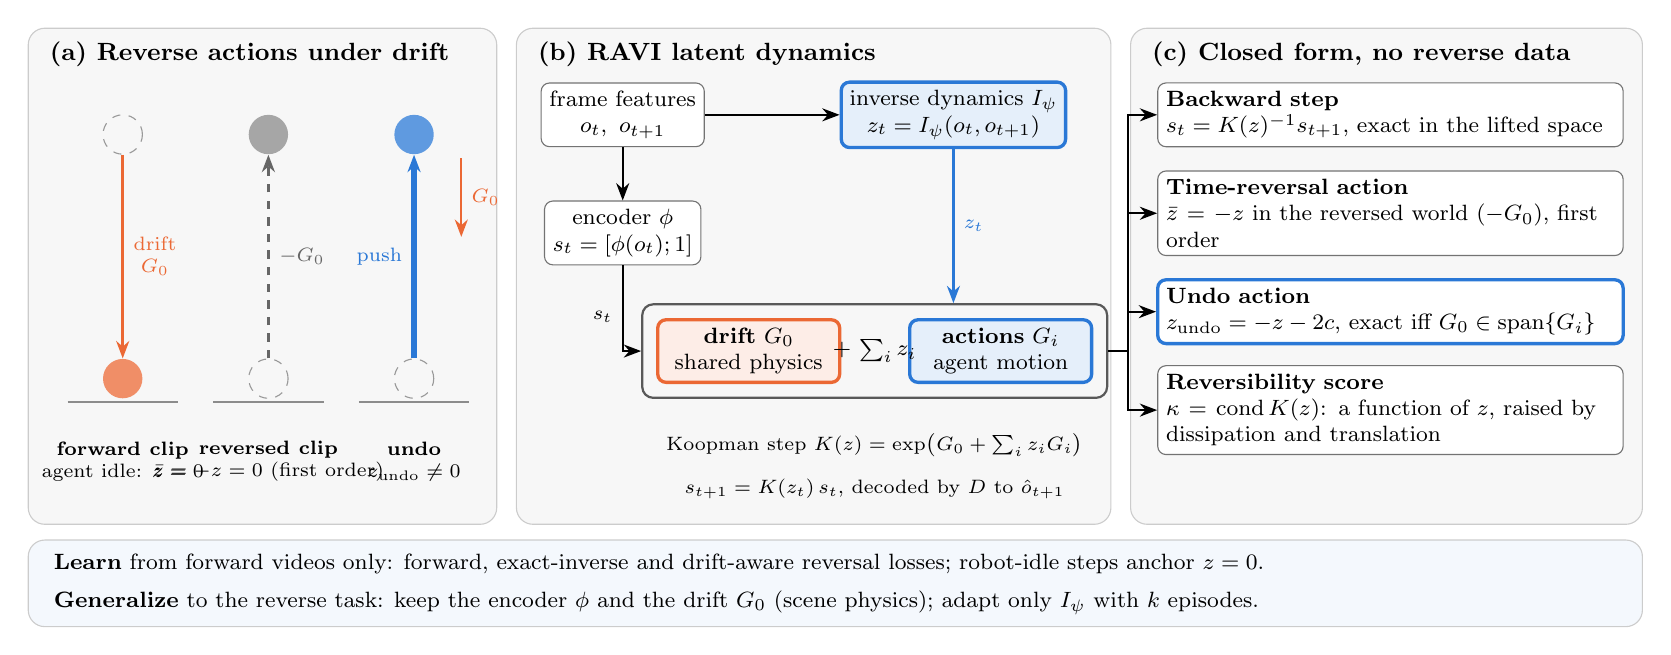
\begin{tikzpicture}[
	font=\footnotesize, >={Stealth[length=2.2mm]},
	box/.style={draw=black!55, rounded corners=3pt, align=center, inner sep=3pt, fill=white},
	driftbox/.style={box, draw=driftc, fill=driftc!12, very thick, text width=2.1cm},
	actbox/.style={box, draw=actc, fill=actc!12, very thick},
	outbox/.style={box, text width=5.7cm, align=left},
	panel/.style={draw=black!20, fill=black!3, rounded corners=6pt},
	ttl/.style={font=\small\bfseries, anchor=west},
	note/.style={font=\scriptsize, align=center},
	ball/.style={circle, minimum size=5mm, inner sep=0pt},
]
% ---------- panels
\draw[panel] (-0.2,0.75) rectangle (5.75,7.05);
\draw[panel] (6.0,0.75) rectangle (13.55,7.05);
\draw[panel] (13.8,0.75) rectangle (20.3,7.05);
\node[ttl] at (-0.05,6.72) {(a) Reverse actions under drift};
\node[ttl] at (6.15,6.72) {(b) RAVI latent dynamics};
\node[ttl] at (13.95,6.72) {(c) Closed form, no reverse data};

% ---------- (a) a falling object seen three ways
\foreach \x in {1.0,2.85,4.7} { \draw[black!45, thick] (\x-0.7,2.3) -- (\x+0.7,2.3); }
% forward clip: the object falls under drift while the agent is idle
\node[ball, draw=black!40, dashed] (f0) at (1.0,5.7) {};
\node[ball, fill=driftc!75] (f1) at (1.0,2.6) {};
\draw[->, driftc, very thick] (f0) -- node[right, note]{drift\\$G_0$} (f1);
\node[note] at (1.0,1.55) {\textbf{forward clip}\\agent idle: $z=0$};
% reversed clip: rises with zero action under reversed drift
\node[ball, draw=black!40, dashed] (r0) at (2.85,2.6) {};
\node[ball, fill=black!35] (r1) at (2.85,5.7) {};
\draw[->, black!60, very thick, dashed] (r0) -- node[right, note]{$-G_0$} (r1);
\node[note] at (2.85,1.55) {\textbf{reversed clip}\\$\bar z=-z=0$ (first order)};
% undo: the agent must push against the drift
\node[ball, draw=black!40, dashed] (u0) at (4.7,2.6) {};
\node[ball, fill=actc!75] (u1) at (4.7,5.7) {};
\draw[->, actc, line width=2pt] (u0) -- node[left, note]{push} (u1);
\draw[->, driftc, thick] (5.3,5.4) -- node[right, note]{$G_0$} (5.3,4.4);
\node[note] at (4.7,1.55) {\textbf{undo}\\$z_{\mathrm{undo}}\neq0$};

% ---------- (b) model
\node[box] (frames) at (7.35,5.95) {frame features\\$o_t,\ o_{t+1}$};
\node[box] (enc) at (7.35,4.45) {encoder $\phi$\\$s_t=[\phi(o_t);1]$};
\node[actbox] (idm) at (11.55,5.95) {inverse dynamics $I_\psi$\\$z_t=I_\psi(o_t,o_{t+1})$};
\node[driftbox] (g0) at (8.95,2.95) {\textbf{drift} $G_0$\\shared physics};
\node[actbox, text width=2.1cm] (gi) at (12.15,2.95) {\textbf{actions} $G_i$\\agent motion};
\node[font=\footnotesize] (plus) at (10.55,2.95) {$+\,\sum_i z_i$};
\node[draw=black!65, rounded corners=4pt, thick, fit=(g0)(gi)(plus), inner sep=5pt] (K) {};
\node[note] at (10.55,1.75) {Koopman step $K(z)=\exp\!\big(G_0+\sum_i z_iG_i\big)$};
\node[note] at (10.55,1.2) {$s_{t+1}=K(z_t)\,s_t$, decoded by $D$ to $\hat o_{t+1}$};
\draw[->, thick] (frames) -- (enc);
\draw[->, thick] (frames) -- (idm);
\draw[->, thick] (enc.south) |- node[pos=0.3, left, note]{$s_t$} (K.west);
\draw[->, thick, actc] (idm.south) -- node[right, note]{$z_t$} (idm.south |- K.north);

% ---------- (c) outputs
\node[outbox] (o1) at (17.1,5.95) {\textbf{Backward step}\\$s_t=K(z)^{-1}s_{t+1}$, exact in the lifted space};
\node[outbox] (o2) at (17.1,4.7) {\textbf{Time-reversal action}\\$\bar z=-z$ in the reversed world ($-G_0$), first order};
\node[outbox, draw=actc, very thick] (o3) at (17.1,3.45) {\textbf{Undo action}\\$z_{\mathrm{undo}}=-z-2c$, exact iff $G_0\in\mathrm{span}\{G_i\}$};
\node[outbox] (o4) at (17.1,2.2) {\textbf{Reversibility score}\\$\kappa=\mathrm{cond}\,K(z)$: a function of $z$, raised by dissipation and translation};
\coordinate (bus) at ($(K.east)+(0.25,0)$);
\draw[thick] (K.east) -- (bus);
\foreach \o in {o1,o2,o3,o4} { \draw[->, thick] (bus) |- (\o.west); }

% ---------- bottom strip: learning and generalization
\draw[panel, fill=actc!5] (-0.2,-0.55) rectangle (20.3,0.55);
\node[anchor=west] at (0.0,0.25) {\textbf{Learn} from forward videos only: forward, exact-inverse and drift-aware reversal losses; robot-idle steps anchor $z=0$.};
\node[anchor=west] at (0.0,-0.25) {\textbf{Generalize} to the reverse task: keep the encoder $\phi$ and the drift $G_0$ (scene physics); adapt only $I_\psi$ with $k$ episodes.};
\end{tikzpicture}}
\caption{RAVI. (a) Under drift, the reversed clip needs no action but the real-world undo does. (b) A Koopman step with drift $G_0$ (shared physics) separate from action generators $G_i$. (c) Reverse quantities in closed form. The design is task-independent; Section~\ref{s:setup} gives the instantiation used here.}
\label{f:concept}
\end{figure*}

{\method} fits a single latent dynamics model to forward footage and reads every reverse quantity off it (Fig.~\ref{f:concept}).
A task and its reverse, such as loading and unloading a toaster, share scene states and physics but not the agent's motion, so the encoder and the drift are shared and only the latent actions are task specific.

\subsection{Lifted State and Drift-Aware Dynamics}
A frozen visual backbone provides features $o_t$ (Section~\ref{s:setup}). A trainable head $\phi$ and a constant coordinate form the lifted state, and the IDM $I_\psi$, which receives $[o_t,o_{t+1},o_{t+1}-o_t]$, produces the latent action:
\begin{equation}
s_t=[\phi(o_t);1]\in\R^{d+1},\qquad z_t=I_\psi(o_t,o_{t+1})\in\R^{m}.
\label{e:state}
\end{equation}
The constant coordinate makes translations linear and keeps the constant observable, which is a Koopman eigenfunction with eigenvalue 1, and we write $x_t=\phi(o_t)$.
Each step is $s_{t+1}=K(z_t)\,s_t$ with Eq.~(\ref{e:koopman}) and the generators
\begin{align}
G_0&=\begin{bmatrix} S-S^\top-LL^\top & b_0\\ 0 & 0\end{bmatrix},\nonumber\\
G_i&=\begin{bmatrix} W_i-W_i^\top+\sym(V_i) & b_i\\ 0 & 0\end{bmatrix},
\label{e:gens}
\end{align}
where $\sym(V)=(V+V^\top)/2$ and the zero last row keeps the constant coordinate at 1.
Each action generator combines a skew block, a weakly L2-penalised symmetric block and a translation, keeping pure actions close to rigid motions, while the drift adds a negative semidefinite part $-LL^\top$ for dissipation such as falling, friction and settling; $M(z)$ is the upper-left $d\times d$ block of $A(z)=G_0+\sum_iz_iG_i$.

\subsection{Reverse Quantities}
\textbf{Backward step.} Because every step is exactly invertible (Proposition~\ref{p:inverse}), the previous state follows without extra parameters,
\begin{equation}
s_t=e^{-A(z_t)}\,s_{t+1},\qquad A(z_t)=G_0+\textstyle\sum_iz_{t,i}G_i.
\label{e:backward}
\end{equation}
and once decoded through $D$ it is as accurate as the forward model.

\textbf{Time-reversal action.} Time reversal negates the drift but keeps the action generators, so $\zb=-z$ explains the reversed clip (Definition~\ref{d:trev}, Proposition~\ref{p:trev}).

\textbf{Undo action.} To undo a step from every state under forward-time dynamics, an action $z'$ must satisfy $G_0+\sum_iz'_iG_i=-(G_0+\sum_iz_iG_i)$, which leads to
\begin{align}
\zundo&=-z-2c,\nonumber\\
c&=\arg\min_c\ \mathbb{E}_{s\sim\mathcal{D}}\Big\|\Big(G_0-\sum_ic_iG_i\Big)s\Big\|^2,
\label{e:undo}
\end{align}
where $c$ imitates the drift on the visited states $\mathcal{D}$.
We fit $c$ on states because $m=16$ generators cannot span all $65\times65$ matrices but may still offset the drift where the robot goes.
For a single transition a weaker condition suffices, and we compute the state-specific undo action
\begin{equation}
\zss_t=\arg\min_{z'}\big\|D\big(K(z')\,s_{t+1}\big)-o_t\big\|^2,
\label{e:undoss}
\end{equation}
by gradient descent from $-z_t-2c$; to first order this is a linear least-squares problem (Proposition~\ref{p:undo}(d)), and an $H$-step plan optimises $H$ actions jointly.
The normalised residual
\begin{equation}
\varepsilon=\frac{\big(\mathbb{E}_s\|(G_0-\sum_ic_iG_i)s\|^2\big)^{1/2}}{\big(\mathbb{E}_s\|G_0s\|^2\big)^{1/2}}
\label{e:residual}
\end{equation}
measures the part of the drift that no state-independent action can cancel and controls the first-order undo error (Proposition~\ref{p:undo}), while the per-transition residual $\varepsilon_t=\|(G_0-\sum_ic_iG_i)s_t\|/\|G_0s_t\|$ localises it.
A residual near 1 must be read against Remark~\ref{r:eps}, because unrelated actions and drift also produce it.

\textbf{Reversibility score.} The condition number $\kappa_t=\cond(K(z_t))=\sigma_{\max}/\sigma_{\min}$ exceeds 1 only through the symmetric part of the generator (Proposition~\ref{p:kappa}), that is, through dissipative drift, symmetric action blocks and translations.
Since $\kappa_t$ depends on the transition only through $z_t$ and grows with translations (Corollary~\ref{c:kappa}), we also evaluate the translation-free score $\klin_t=\cond(e^{M(z_t)})$ and the state-dependent contraction rate $\rho_t=\|L^\top x_t\|^2/\|x_t\|^2$.

\subsection{Anchoring the Agent/Drift Split} \label{s:anchor}
The shift $z\to z+c$, $G_0\to G_0-\sum_ic_iG_i$ leaves every prediction unchanged (Proposition~\ref{p:gauge}), so {\method} fixes it by requiring $z_t\approx0$ on robot-idle steps $\mathcal{N}$, which are identified from proprioceptive joint speed.
The anchor uses no action labels, but because joint speed is not visual, only {\method} without the anchor is trained from video alone.

\subsection{Training Objective}
With a decoder $D$ and the reversed latent action $\zb_t=I_\psi(o_{t+1},o_t)$, {\method} minimises
\begin{align}
\mathcal{L}&=\ell_{\mathrm{fwd}}+\lambda_b\,\ell_{\mathrm{bwd}}+\lambda_r\,(\ell_{\mathrm{rev}}+\ell_{\mathrm{neg}})\nonumber\\
&\quad+\lambda_a\,\ell_{\mathrm{idle}}+\lambda_v\,\Omega+\mathcal{L}_{\mathrm{rec}},\nonumber\\
\ell_{\mathrm{fwd}}&=\big\|o_{t+1}-D\big(e^{A(z_t)}s_t\big)\big\|^2,\nonumber\\
\ell_{\mathrm{bwd}}&=\big\|o_t-D\big(e^{-A(z_t)}s_{t+1}\big)\big\|^2,\nonumber\\
\ell_{\mathrm{rev}}&=\big\|o_t-D\big(e^{-G_0+\sum_i\zb_{t,i}G_i}s_{t+1}\big)\big\|^2,\nonumber\\
\ell_{\mathrm{neg}}&=\|z_t+\zb_t\|^2,\quad \ell_{\mathrm{idle}}=\textstyle\sum_{t\in\mathcal{N}}\|z_t\|^2,\nonumber\\
\Omega&=\textstyle\sum_i\|V_i\|_F^2,
\label{e:loss}
\end{align}
where $\mathcal{L}_{\mathrm{rec}}$ reconstructs $o_t$ and $o_{t+1}$ from their lifted states and includes $\|K(z_t)s_t-s_{t+1}\|^2$.
Together, $\ell_{\mathrm{rev}}$ and $\ell_{\mathrm{neg}}$ form the \emph{drift-aware reversal loss}, which decodes the swapped pair under $-G_0$ where sign-reversal losses~\cite{tang2026alam} keep $+G_0$; in practice it enforces IDM antisymmetry (Remark~\ref{r:reduce}). Algorithm~\ref{a:wao} summarises training and the reverse quantities.

\begin{algorithm}[t]
\caption{{\method}: training and reverse quantities}\label{a:wao}
\begin{algorithmic}[1]
\Require forward videos, idle set $\mathcal{N}$, weights $\lambda_b,\lambda_r,\lambda_a,\lambda_v$
\Repeat
	\State sample transitions $(o_t,o_{t+1})$ with idle flags
	\State $s_t\gets[\phi(o_t);1]$, $s_{t+1}\gets[\phi(o_{t+1});1]$
	\State build $G_0$, $G_i$ by Eq.~(\ref{e:gens})
	\State $z\gets I_\psi(o_t,o_{t+1})$, $\zb\gets I_\psi(o_{t+1},o_t)$
	\State $A\gets G_0+\sum_iz_iG_i$
	\State $L_{\mathrm{fwd}}\gets\|D(e^{A}s_t)-o_{t+1}\|^2$
	\State $L_{\mathrm{bwd}}\gets\|D(e^{-A}s_{t+1})-o_t\|^2$
	\State $L_{\mathrm{rev}}\gets\|D(e^{-G_0+\sum_i\zb_iG_i}s_{t+1})-o_t\|^2+\|\zb+z\|^2$
	\State update all parameters on Eq.~(\ref{e:loss})
\Until{converged}
\State $c\gets\arg\min_c\mathbb{E}_s\|(G_0-\sum_ic_iG_i)s\|^2$; $\varepsilon\gets$ Eq.~(\ref{e:residual})
\For{each forward transition $t$}
	\State $s_t\gets e^{-A_t}s_{t+1}$ \Comment{backward step}
	\State $\zb_t\gets-z_t$ \Comment{time-reversal action}
	\State $z_{\mathrm{undo},t}\gets-z_t-2c$ \Comment{undo, all states}
	\State $\zss_t\gets$ Eq.~(\ref{e:undoss}) from $-z_t-2c$ \Comment{undo, this state}
	\State $\kappa_t\gets\cond(e^{A_t})$, $\klin_t\gets\cond(e^{M_t})$ \Comment{scores}
	\State $\rho_t\gets\|L^\top x_t\|^2/\|x_t\|^2$ \Comment{state-dependent}
\EndFor
\State \textbf{return} $(z_{\mathrm{undo},T-1},\dots,z_{\mathrm{undo},1})$, $\{\zss_t\}$, $\{\kappa_t,\klin_t,\rho_t\}$, $\varepsilon$
\end{algorithmic}
\end{algorithm}

\subsection{Transfer between Forward and Reverse Tasks}
From insertion data alone, and symmetrically from removal, {\method} forecasts removal by playing the insertion undo actions backward, compares them with the IDM's actions on real removal clips, and adapts from $k$ episodes by fine-tuning only the IDM, keeping $G_0$ and $\phi$ frozen because the physics does not change (Section~\ref{s:results} also tunes $G_0$). Where real reverse motion departs from the derived undo, as when a slice is lifted out, the residual and the undo error flag it.

\textbf{Practical cost.} Every forward step evaluates one $(d+1)\times(d+1)$ matrix exponential by scaling and squaring, at a cost of $O(d^3)$ that is negligible for $d=64$, and the backward step reuses the same exponent with the opposite sign. The time-reversal action, the undo action, the residual and the reversibility scores need no further training once the forward model is fitted; only the state-specific undo solves a small optimisation over $m=16$ variables per transition. A complete cross-validation run, including all diagnostics, therefore takes about four minutes on one GPU.

% =====================================================================
\section{Theoretical Analysis} \label{s:theory}

This section establishes the properties on which the reverse quantities rest. We first connect the model to control-affine dynamics (Proposition~\ref{p:affine}), then show that every step is exactly invertible and that the time-reversal action needs no commuting generators (Propositions~\ref{p:inverse} and~\ref{p:trev}), characterise when a step can be undone (Proposition~\ref{p:undo}), and finally explain why the agent/drift split must be anchored, why sign reversal forces zero drift and what the reversibility score measures (Propositions~\ref{p:gauge}--\ref{p:kappa} and Corollary~\ref{c:kappa}).
We write $A(z)=G_0+\sum_iz_iG_i$ and $K(z)=\exp(A(z))$.
For a square matrix $X$, $X_s=(X+X^\top)/2$ is its symmetric part.

\begin{proposition}[Affine Koopman generator]
\label{p:affine}
For the control-affine system~(\ref{e:cas}) with constant input $u$, the Koopman generator $\mathcal{L}_u g=\nabla g\cdot(f+\sum_iu_ig_i)$ satisfies $\mathcal{L}_u=\mathcal{L}_f+\sum_iu_i\mathcal{L}_{g_i}$, and the step operator over $\Delta t$ is $\exp(\Delta t\,\mathcal{L}_u)$.
\end{proposition}
\begin{proof}
For a differentiable observable $g$, $\mathcal{L}_ug=\frac{d}{dt}g(s(t))=\nabla g\cdot\dot s=\nabla g\cdot f+\sum_iu_i\,\nabla g\cdot g_i$, which is $\mathcal{L}_fg+\sum_iu_i\mathcal{L}_{g_i}g$.
With $u$ constant over the step, the flow is autonomous and the Koopman semigroup is generated by $\mathcal{L}_u$, giving $\exp(\Delta t\,\mathcal{L}_u)$.
\end{proof}
This standard property~\cite{goswami2017global,bruder2021bilinear} fixes notation. Eq.~(\ref{e:koopman}) restricts it to the learned observables, with $G_0$ in the role of $\Delta t\,\mathcal{L}_f$ and $G_i$ in that of $\Delta t\,\mathcal{L}_{g_i}$, and the restriction is exact only if their span is invariant and the input is constant over the step, both of which are modelling assumptions.

\begin{proposition}[Exact inverse]
\label{p:inverse}
For every $z$, $K(z)$ is invertible with $K(z)^{-1}=\exp(-A(z))$, and $\det K(z)=e^{\mathrm{tr}\,A(z)}>0$.
\end{proposition}
\begin{proof}
$A$ and $-A$ commute, so $\exp(A)\exp(-A)=\exp(A-A)=I$.
The determinant identity $\det\exp(A)=e^{\mathrm{tr}A}$ follows from the Jordan form of $A$.
\end{proof}
The backward step~(\ref{e:backward}) is thus the exact inverse of the learned step, with no extra parameters, and as accurate as the forward model (Section~\ref{s:results}).

\begin{proposition}[Time-reversal action]
\label{p:trev}
In the reversed world with drift $-G_0$ and unchanged action generators, define $\bar K(\zb)=\exp(-G_0+\sum_i\zb_iG_i)$.
Then $\bar K(-z)=K(z)^{-1}$ for every $z$, so the action $\zb=-z$ reproduces the reversed transition $s_{t+1}\to s_t$ exactly.
No commutativity among $G_0,G_1,\dots,G_m$ is required.
\end{proposition}
\begin{proof}
$\bar K(-z)=\exp(-G_0-\sum_iz_iG_i)=\exp(-A(z))=K(z)^{-1}$ by Proposition~\ref{p:inverse}.
Only one exponential of a single sum appears, so no product of exponentials of non-commuting matrices is involved.
\end{proof}
Its content lies in Definition~\ref{d:trev}, which takes the reversed world as the time reversal of the first-order latent dynamics.

\begin{remark}
Composition differs: by the Baker--Campbell--Hausdorff formula, $K(z_2)K(z_1)=K(z_1+z_2)$ only for commuting generators, so additive composition~\cite{wei2026aclam} is an abelian assumption, whereas $\zb=-z$ is not.
\end{remark}

\begin{remark}[Reduction of the drift-aware reversal loss]
\label{r:reduce}
If $\zb_t=-z_t$, then $e^{-G_0+\sum_i\zb_{t,i}G_i}=K(z_t)^{-1}$ by Proposition~\ref{p:trev}, so $\ell_{\mathrm{rev}}=\ell_{\mathrm{bwd}}$ in Eq.~(\ref{e:loss}).
The loss therefore adds only IDM antisymmetry, $I_\psi(o_{t+1},o_t)=-I_\psi(o_t,o_{t+1})$, to exact-inverse reconstruction.
What keeps drift out of the action is the operator form: decoding swapped pairs under $+G_0$ is incompatible with any drift (Proposition~\ref{p:signrev}), whereas decoding them under $-G_0$ is compatible with every $G_0$, and the ablation {\method}-SR isolates this difference.
\end{remark}

\begin{proposition}[Undo action]
\label{p:undo}
Let $\mathcal{G}=\mathrm{span}\{G_1,\dots,G_m\}$.
(a) If $G_0=\sum_ic_iG_i\in\mathcal{G}$, then $\zundo=-z-2c$ satisfies $K(\zundo)K(z)=I$, an exact single-step undo for every state.
(b) \emph{State-independent undo.} Suppose $K(z')K(z)=I$, i.e.\ $z'$ undoes the step from every state, and the spectra of $A(z)$ and $A(z')$ lie in the strip $|\mathrm{Im}\,\lambda|<\pi$. Then $A(z')=-A(z)$, which is possible only if $G_0\in\mathcal{G}$.
(c) For any $c$, $K(-z-2c)K(z)s=s+2(G_0-\sum_ic_iG_i)s+O(\|A\|^2)\,\|s\|$, where $\|A\|=\max(\|A(z)\|,\|A(-z-2c)\|)$; the first-order undo error is twice the uncancelled drift, whose relative size on visited states is $\varepsilon$ in Eq.~(\ref{e:residual}).
(d) \emph{State-specific undo, first order.} For a transition $s_t\to s_{t+1}$ let $B_t=[G_1s_{t+1},\dots,G_ms_{t+1}]$ and $r_t=s_t-s_{t+1}-G_0s_{t+1}$. Then $K(z')s_{t+1}-s_t=B_tz'-r_t+O(\|A(z')\|^2)\,\|s_{t+1}\|$; a first-order undo of this transition exists if and only if $r_t\in\mathrm{range}(B_t)$, and $z'=B_t^{+}r_t$ minimises its first-order error.
\end{proposition}
\begin{proof}
(a) $A(-z-2c)=G_0-\sum_i(z_i+2c_i)G_i=G_0-2G_0-\sum_iz_iG_i=-A(z)$, so $K(\zundo)K(z)=\exp(-A)\exp(A)=I$.
(b) $K(z')K(z)=I$ gives $\exp(A(z'))=\exp(-A(z))$.
On matrices whose spectra lie in the strip, the matrix exponential is injective (the principal logarithm is unique~\cite{higham2008functions}), so $A(z')=-A(z)$, i.e.\ $\sum_i(z'_i+z_i)G_i=-2G_0$, which requires $G_0\in\mathcal{G}$.
(c) For matrices $X,Y$, the series of the exponential gives $e^Xe^Y=I+X+Y+O(\max(\|X\|,\|Y\|)^2)$.
With $X=A(-z-2c)=G_0-\sum_i(z_i+2c_i)G_i$ and $Y=A(z)=G_0+\sum_iz_iG_i$, we have $X+Y=2G_0-2\sum_ic_iG_i=2\big(G_0-\sum_ic_iG_i\big)$.
Applying both sides to $s$ gives the claim.
Taking expectations over visited states, the first-order undo error relative to $\|G_0s\|$ is $2\varepsilon$, so $c$ in Eq.~(\ref{e:undo}) minimises it.
(d) $K(z')s_{t+1}=s_{t+1}+A(z')s_{t+1}+O(\|A(z')\|^2)\|s_{t+1}\|$ and $A(z')s_{t+1}=G_0s_{t+1}+B_tz'$; subtracting $s_t$ gives the expansion, and the rest is linear least squares.
\end{proof}
Part~(b) concerns undo from every state, which is what a single $c$ provides, and does not exclude state-specific undo, for which part~(d) only requires the displacement at $s_{t+1}$ to lie in the at most $m$-dimensional range of $B_t$.
Both (c) and (d) need a small $\|A\|$, which Section~\ref{s:results} checks.

\begin{remark}[Reference value for the drift residual]
\label{r:eps}
For a state $s=[x;1]$, the vectors $G_is$ span a subspace $U_s$ of dimension at most $m$ within the $d$ coordinates of $x$.
If $G_0s$ were isotropic given $U_s$, with $\mathbb{E}[G_0s\,(G_0s)^\top\mid U_s]=\sigma^2I$, even a state-dependent $c$ would leave $\mathbb{E}\|P_{U_s^\perp}G_0s\|^2\ge(1-m/d)\,\mathbb{E}\|G_0s\|^2$, i.e.\ $\varepsilon\ge(1-m/d)^{1/2}\approx0.87$ for $m=16$ and $d=64$; a single $c$ shared across states leaves more.
Moreover, the dissipative block contributes $x^\top(-LL^\top)x=-\|L^\top x\|^2$ along $x$, which skew blocks cannot produce ($x^\top(W-W^\top)x=0$); only the penalised symmetric blocks and translations can.
A residual near 1 is thus expected when actions and drift are unrelated; it shows that the actions cannot cancel the drift, not that a given event, such as a drop, is irreversible.
\end{remark}

\begin{proposition}[Non-identifiability of the agent/drift split]
\label{p:gauge}
For any $c\in\R^m$, the transformation $z\to z+c$, $G_0\to G_0-\sum_ic_iG_i$ leaves $A(z_t)$, and hence every forward prediction, unchanged.
The split between agent effects and drift is therefore not identifiable from action-free video.
\end{proposition}
\begin{proof}
$G_0-\sum_ic_iG_i+\sum_i(z_i+c_i)G_i=G_0+\sum_iz_iG_i$, so $A(z_t)$ and $K(z_t)$ are the same for every transition, and so is every prediction made from them.
\end{proof}
The residuals $\varepsilon$ and $\varepsilon_t$ are invariant, since Eq.~(\ref{e:undo}) absorbs any shift of $G_0$ within $\mathcal{G}$, but the reversed world is not, because $-G_0$ changes with $c$; the zero action must therefore be fixed, here by idle transitions (Section~\ref{s:anchor}) and otherwise by a few labels.

\begin{proposition}[Sign reversal forces zero drift]
\label{p:signrev}
Consider a sign-reversal model that decodes swapped pairs with the forward operator and $\zb=-z$, i.e.\ $s_t=K(-z)s_{t+1}$.
If this is consistent with the forward step $s_{t+1}=K(z)s_t$ on a set of states that spans $\R^{d+1}$, and the spectra of $A(z)$ and $A(-z)$ lie in the strip $|\mathrm{Im}\,\lambda|<\pi$, then $G_0=0$.
\end{proposition}
\begin{proof}
Consistency on a spanning set gives $K(-z)K(z)=I$, i.e.\ $\exp(G_0-\sum_iz_iG_i)=\exp(-G_0-\sum_iz_iG_i)$.
By injectivity of the exponential on the strip, $G_0-\sum_iz_iG_i=-G_0-\sum_iz_iG_i$, hence $G_0=0$.
\end{proof}
An exactly consistent Koopman sign-reversal model thus leaves all passive dynamics to the latent action, which is the drift absorption that the drift-aware loss avoids, since by Proposition~\ref{p:trev} that loss is consistent for any $G_0$.
The result does not cover nonlinear forward models, in which a state-dependent action can absorb drift without contradiction, so it applies to {\method}-SR but not to the MLP sign-reversal baseline.

\begin{proposition}[Reversibility score]
\label{p:kappa}
For any real square $A$, $\sigma_{\max}(e^A)\le e^{\lambda_{\max}(A_s)}$ and $\sigma_{\min}(e^A)\ge e^{\lambda_{\min}(A_s)}$, hence
\begin{equation}
\cond(e^A)\le\exp\big(\lambda_{\max}(A_s)-\lambda_{\min}(A_s)\big).
\label{e:kappa}
\end{equation}
In particular, if $A$ is skew-symmetric then $e^A$ is orthogonal and $\cond(e^A)=1$.
\end{proposition}
\begin{proof}
The logarithmic norm in the spectral norm is $\mu(A)=\lambda_{\max}(A_s)$, and $\|e^{A}\|_2\le e^{\mu(A)}$ (Dahlquist's bound, obtained from $\frac{d}{dt}\|e^{tA}x\|^2=2x^\top e^{tA^\top}A_se^{tA}x\le2\mu(A)\|e^{tA}x\|^2$).
Applying the same bound to $-A$ gives $\sigma_{\min}(e^A)=1/\|e^{-A}\|_2\ge e^{-\mu(-A)}=e^{\lambda_{\min}(A_s)}$.
If $A^\top=-A$, then $(e^A)^\top e^A=e^{-A}e^A=I$.
\end{proof}
In {\method}, $A_s$ collects $-LL^\top$, the symmetric action blocks and the translations, so a large $\kappa_t$ marks a dissipative, non-rigid or translating step, where inversion amplifies error.

\begin{corollary}[What $\kappa_t$ measures]
\label{c:kappa}
(i) $\kappa_t=\cond(K(z_t))$ depends on the transition only through $z_t$: $G_0$ enters as the same matrix at every step, so a passive event that leaves $z_t$ unchanged leaves $\kappa_t$ unchanged.
(ii) For $A=\begin{bmatrix}M&b\\0&0\end{bmatrix}$, $e^A=\begin{bmatrix}e^M&\varphi(M)b\\0&1\end{bmatrix}$ with $\varphi(M)=\sum_{k\ge0}M^k/(k+1)!$.
In particular a pure translation ($M=0$, $b\neq0$) has $\cond(e^A)>1$, so translations of the lifted state raise $\kappa_t$, whereas $\klin_t=\cond(e^{M(z_t)})$ is unaffected by them.
\end{corollary}
\begin{proof}
(i) $\kappa_t$ is a function of $A(z_t)=G_0+\sum_iz_{t,i}G_i$, in which only $z_t$ varies.
(ii) For $k\ge1$, $A^k=\begin{bmatrix}M^k&M^{k-1}b\\0&0\end{bmatrix}$, and summing the exponential series gives the stated form.
For $M=0$, $e^A=\begin{bmatrix}I&b\\0&1\end{bmatrix}$ has determinant 1 and a last column of norm $(1+\|b\|^2)^{1/2}>1$, so it is not orthogonal; its singular values multiply to 1 and are not all 1, hence $\sigma_{\max}>1>\sigma_{\min}$.
\end{proof}
Hence $\kappa_t$ can flag a drop only through what the IDM writes into $z_t$, either the release motion or absorbed drift. The state-dependent $\rho_t$ avoids this limitation, although the learned $L$ need not contract where the scene actually settles (Section~\ref{s:toy}).

% =====================================================================
\section{Experimental Setup} \label{s:setup}

\begin{figure*}[t]
	\centering
	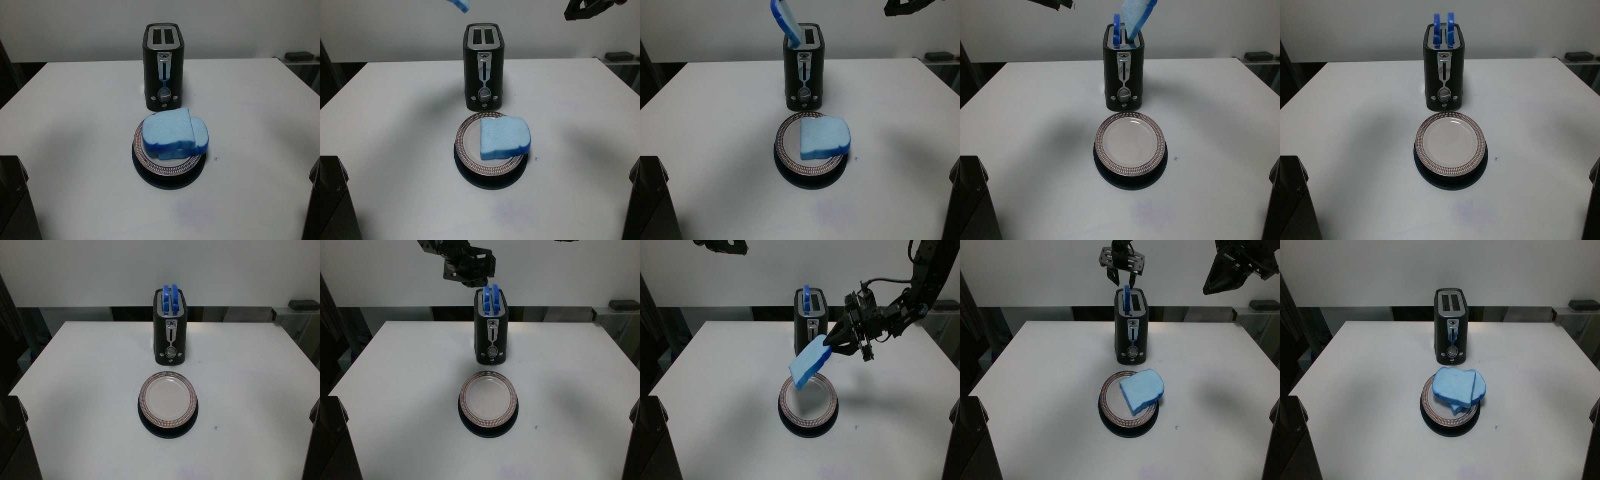
\includegraphics[width=\textwidth]{figs/fig_dataset.jpg}
	\caption{ALOHA toaster task, top camera. Top: insertion (slices dropped into the slots). Bottom: removal (slices returned to the plate).}
	\label{f:dataset}
\end{figure*}

\subsection{Data}
ALOHA~\cite{zhao2023aloha} has two 6-DoF arms with parallel grippers and logs 14-D joint actions at 50\,Hz with three $480\times848$ RGB streams, one overhead and one per wrist.
We use 50 \textbf{insertion} and 50 \textbf{removal} recordings of 25\,s (Fig.~\ref{f:dataset}; one insertion without motion was excluded), which visit the same three scene states in opposite order: both slices on the plate, one in the toaster, and both in the toaster.
Carrying a grasped slice is quasi-static and almost reversible, whereas the drop into a slot, triggered by opening the gripper and complete within a fraction of a 0.5\,s step, is not, and otherwise the scene is static unless the robot moves it.
Features are computed at 10\,Hz and one step covers 0.5\,s, with all five phase offsets used for training and offset 0 for evaluation in 5-fold cross-validation over whole recordings.
Training never sees joint actions, and joint speed is used only to define the anchor set $\mathcal{N}$ as the slowest 15\% of steps.
Gripper positions only locate releases for evaluation, defined as an opening beyond 0.9 after holding ($0.05<g<0.9$) for at least 1\,s; this rule finds exactly two releases in 41 of 50 insertion and 49 of 50 removal recordings and yields 93 post-release against 810 carrying steps for insertion and 103 against 898 for removal.

\subsection{Representation and Training}
Top-camera frames, resized to $224\times392$, are encoded by a frozen DINOv2 ViT-S/14~\cite{oquab2024dinov2}. The CLS token (384-D) and a $2\times4$ pooled patch grid (3,072-D) are standardised and reduced by PCA, fitted on training episodes, to the 128-D features $o_t$ in which all reconstruction and errors are measured, and a linear probe decodes the three scene stages from these features with 97.5\% balanced accuracy (chance 33.3\%).
The head $\phi$ and the decoder are two-layer MLPs with 256 hidden units, $d=64$ and $m=16$, and $K(z)$ uses a batched scaling-and-squaring exponential~\cite{higham2005scaling}.
All models share the encoder, the decoder and the training budget of 4,000 Adam updates with batch size 512 and learning rate $10^{-3}$, with $\lambda_b=\lambda_r=\lambda_a=1$ and $\lambda_v=10^{-3}$; one run takes about four minutes on an A100.
Every model is trained with three seeds per fold, so each descriptive robot-data value is a mean over 15 runs per model and direction, and rerunning seed 0 reproduced the earlier single-seed results exactly. For the tests and the control metrics, every model is also trained once on each of 10 folds (160 runs).

\subsection{Baselines and Ablations}
The \textbf{LAM}~\cite{schmidt2024lapo} has MLP forward and backward models, the latter trained on time-reversed clips, and takes the IDM on the swapped pair as its reverse action.
The \textbf{sign-reversal LAM}~\cite{tang2026alam} instead decodes swapped pairs with one shared MLP forward model and $\zb=-z$, and \textbf{{\method} w/o anchor} drops the anchor.
Three Koopman ablations isolate the drift sign, the reversal loss and the drift itself: \textbf{{\method}-SR} decodes swapped pairs under $+G_0$ and is the model of Proposition~\ref{p:signrev}, \textbf{{\method} w/o reversal} sets $\lambda_r=0$, and \textbf{{\method}, $G_0=0$} has no drift generator.
Finally, the \textbf{two-direction reference} is {\method} trained on both directions. Because it sees the test task and, for rollouts and alignment, uses the IDM's actions on the test recording itself, it is a reference rather than an upper bound.

\subsection{Evaluation Protocol}
Models trained on insertion are tested on removal (I$\to$R) and vice versa (R$\to$I), and errors are relative to predicting no change, $\|\hat o-o\|^2/\|o_{\mathrm{prev}}-o\|^2$, so that 1.0 equals copying the current frame.
The \textbf{forward and backward errors} on held-out training-direction recordings measure reconstruction rather than open-loop prediction, since the IDM sees $o_{t+1}$.
To test the reverse actions, we roll out those derived from a held-out training recording from a test recording of the opposite task and report the \textbf{end-distance ratio}, the final over the initial distance to the target-stage prototype in decoded features.
Because decoding alone can contract a rollout, null rollouts use zero actions, random actions from a Gaussian fitted to the training actions, and unreversed forward actions, and we also divide each model's ratio by that of its own zero-action rollout (\textbf{end distance relative to null}, below 1 when the actions help) and measure it from the decoded rather than the observed start.
\textbf{Action alignment} is the cosine between derived and real reverse actions after time warping, against a time-permuted reference, and the \textbf{joint-probe error} maps $z$ linearly to 14-D joint deltas, against negated, time-reversed deltas.

The \textbf{reversibility AUROC} measures how well $\kappa_t$ separates the 0.5\,s after each release from grasped carrying on held-out recordings of the training direction, that is, drops into the slots for I$\to$R and placements on the plate for R$\to$I; for the LAM baselines we use the condition number of the forward-model Jacobian, which, unlike $\kappa_t$, depends on the state.
We also score $\klin_t$, $\rho_t$, $\varepsilon_t$, the \textbf{inverse-step error} $\|D(K(z_t)^{-1}s_{t+1})-o_t\|$, which uses the state as well as the action, in absolute terms and divided by the step length, and four simple detectors, $\|z_t\|$, the feature change $\|o_{t+1}-o_t\|$, arm joint speed and a gripper-opening indicator, both against all carrying steps and against matched carrying steps, the three nearest to each post-release step in arm speed, which reflects the agent's motion, or in feature change, which reflects the total motion.
The \textbf{few-shot error} is the opposite-task error after fine-tuning the IDM, or the IDM and $G_0$, on $k\in\{0,1,3,5\}$ recordings, and the \textbf{drift residual} $\varepsilon$ is compared with Remark~\ref{r:eps} and with a random $G_0$ of equal structure and norm.
\textbf{Undo success} is the fraction of transitions that the undo~(\ref{e:undoss}) returns within half a step, $\|D(K(\zss_t)s_{t+1})-o_t\|<0.5\,\|o_{t+1}-o_t\|$, in one or three steps, together with the median absolute error in feature units, and \textbf{drift absorption} is the AUROC of a logistic probe from $z_t$ to the post-release label, also after regressing arm joint change, arm speed and gripper change out of $z_t$ on training steps (\textbf{residual absorption}).
Because seeds share their fold's test recordings, the unit of analysis is the fold: Table~\ref{t:paired} uses paired $t$-tests over the 10 folds, equal for this balanced design to a mixed model with fold as random effect, Holm-corrected across its 36 tests.

% =====================================================================
\section{Results} \label{s:results}

\begin{figure*}[t]
	\centering
	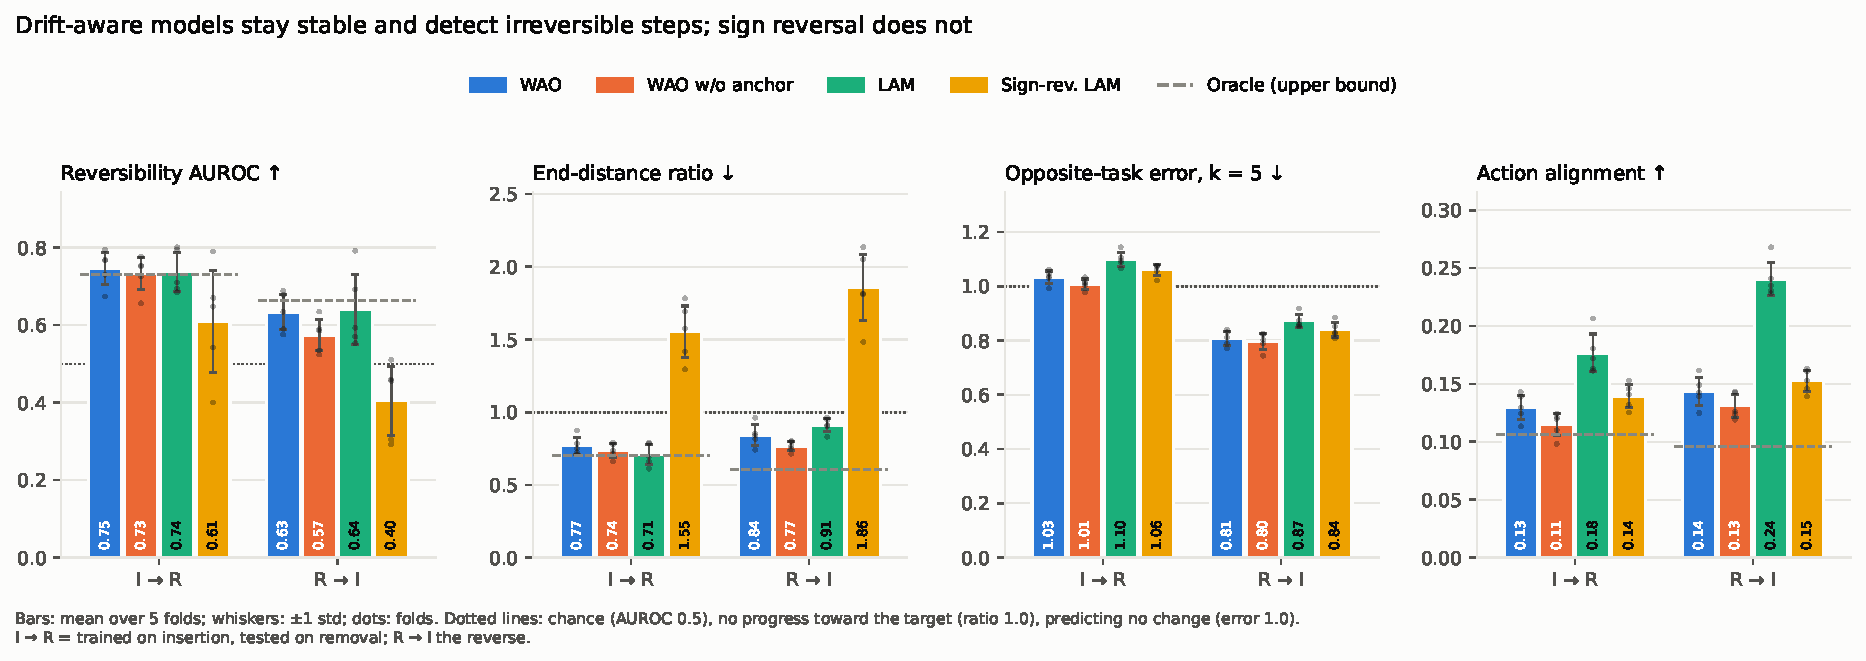
\includegraphics[width=\textwidth]{figs/fig_compare_bars.pdf}
	\caption{Main metrics, mean $\pm$ s.d.\ over 15 runs (dots). Dotted: chance or no-change level; dashed: two-direction reference.}
	\label{f:bars}
\end{figure*}

\begin{table*}
	\centering
	\caption{Cross-validated results, mean $\pm$ s.d.\ over 15 runs (5 folds $\times$ 3 seeds). Bold: best non-reference model.}
	\label{t:main}
	\footnotesize
	\setlength{\tabcolsep}{3.2pt}
	\begin{tabular}{llccccc}
		\toprule
		Metric & Dir. & LAM & Sign-rev. LAM & {\method} w/o anchor & {\method} & Two-dir. ref. \\
		\midrule
		\multirow{2}{*}{Forward error $\downarrow$} & I$\to$R & 0.221$\pm$0.011 & \textbf{0.218}$\pm$0.010 & 0.222$\pm$0.010 & 0.229$\pm$0.010 & 0.225$\pm$0.008 \\
		 & R$\to$I & 0.228$\pm$0.006 & \textbf{0.225}$\pm$0.007 & 0.226$\pm$0.006 & 0.234$\pm$0.006 & 0.237$\pm$0.006 \\
		\multirow{2}{*}{Backward error $\downarrow$} & I$\to$R & 0.225$\pm$0.011 & \textbf{0.221}$\pm$0.010 & 0.225$\pm$0.010 & 0.232$\pm$0.010 & 0.226$\pm$0.008 \\
		 & R$\to$I & 0.229$\pm$0.007 & \textbf{0.225}$\pm$0.007 & 0.227$\pm$0.006 & 0.235$\pm$0.007 & 0.236$\pm$0.006 \\
		\multirow{2}{*}{End-distance ratio $\downarrow$} & I$\to$R & 0.791$\pm$0.089 & 1.583$\pm$0.278 & \textbf{0.743}$\pm$0.056 & 0.754$\pm$0.057 & 0.707$\pm$0.045 \\
		 & R$\to$I & 0.884$\pm$0.083 & 2.132$\pm$0.468 & \textbf{0.793}$\pm$0.067 & 0.838$\pm$0.056 & 0.599$\pm$0.024 \\
		\multirow{2}{*}{Action alignment $\uparrow$} & I$\to$R & \textbf{0.179}$\pm$0.018 & 0.140$\pm$0.012 & 0.116$\pm$0.010 & 0.133$\pm$0.012 & 0.107$\pm$0.050 \\
		 & R$\to$I & \textbf{0.236}$\pm$0.012 & 0.152$\pm$0.011 & 0.132$\pm$0.010 & 0.145$\pm$0.011 & 0.097$\pm$0.050 \\
		\multirow{2}{*}{Joint-probe error $\downarrow$} & I$\to$R & 1.183$\pm$0.038 & \textbf{1.084}$\pm$0.025 & \textbf{1.084}$\pm$0.023 & 1.090$\pm$0.023 & 1.225$\pm$0.044 \\
		 & R$\to$I & 1.185$\pm$0.044 & \textbf{1.076}$\pm$0.057 & 1.094$\pm$0.061 & 1.103$\pm$0.055 & 1.272$\pm$0.033 \\
		\multirow{2}{*}{Reversibility AUROC $\uparrow$} & I$\to$R & 0.722$\pm$0.063 & 0.617$\pm$0.100 & 0.729$\pm$0.037 & \textbf{0.746}$\pm$0.035 & 0.731$\pm$0.036 \\
		 & R$\to$I & 0.610$\pm$0.094 & 0.402$\pm$0.082 & 0.589$\pm$0.049 & \textbf{0.635}$\pm$0.055 & 0.659$\pm$0.042 \\
		\multirow{2}{*}{Few-shot error, $k=5$ $\downarrow$} & I$\to$R & 1.076$\pm$0.033 & 1.051$\pm$0.030 & \textbf{1.001}$\pm$0.034 & 1.029$\pm$0.038 & -- \\
		 & R$\to$I & 0.868$\pm$0.021 & 0.840$\pm$0.027 & \textbf{0.804}$\pm$0.026 & 0.815$\pm$0.022 & -- \\
		\multirow{2}{*}{Drift residual $\varepsilon$} & I$\to$R & -- & -- & 0.997$\pm$0.001 & 0.988$\pm$0.004 & 0.992$\pm$0.003 \\
		 & R$\to$I & -- & -- & 0.997$\pm$0.001 & 0.990$\pm$0.001 & 0.992$\pm$0.002 \\
		\bottomrule
	\end{tabular}
\end{table*}

\begin{table*}
	\centering
	\caption{Fold-level paired comparison over 10 folds. $\Delta$: {\method} minus the other model (mean $\pm$ s.d.\ over folds); wins: folds in which {\method} is better; $p$: paired $t$-test, Holm-corrected over all 36 tests.}
	\label{t:paired}
	\footnotesize
	\setlength{\tabcolsep}{3.5pt}
	\begin{tabular}{llcccccc}
		\toprule
		& & \multicolumn{3}{c}{I$\to$R} & \multicolumn{3}{c}{R$\to$I} \\
		\cmidrule(r){3-5} \cmidrule(l){6-8}
		Compared with & Metric & $\Delta$ & wins & $p_{\mathrm{Holm}}$ & $\Delta$ & wins & $p_{\mathrm{Holm}}$ \\
		\midrule
		\multirow{3}{*}{LAM} & End-distance ratio $\downarrow$ & -0.062$\pm$0.090 & 7/10 & 0.884 & +0.036$\pm$0.115 & 4/10 & 1.000 \\
		 & Reversibility AUROC $\uparrow$ & +0.062$\pm$0.054 & 9/10 & 0.129 & +0.090$\pm$0.156 & 7/10 & 1.000 \\
		 & Few-shot error, $k=5$ $\downarrow$ & -0.065$\pm$0.036 & 10/10 & 0.009 & -0.047$\pm$0.015 & 10/10 & $<$0.001 \\
		\midrule
		\multirow{3}{*}{Sign-rev. LAM} & End-distance ratio $\downarrow$ & -1.029$\pm$0.576 & 10/10 & 0.009 & -1.044$\pm$0.809 & 10/10 & 0.072 \\
		 & Reversibility AUROC $\uparrow$ & +0.101$\pm$0.093 & 9/10 & 0.170 & +0.197$\pm$0.076 & 10/10 & $<$0.001 \\
		 & Few-shot error, $k=5$ $\downarrow$ & -0.049$\pm$0.029 & 9/10 & 0.015 & -0.015$\pm$0.022 & 7/10 & 0.924 \\
		\midrule
		\multirow{3}{*}{{\method} w/o anchor} & End-distance ratio $\downarrow$ & -0.032$\pm$0.091 & 5/10 & 1.000 & +0.091$\pm$0.074 & 1/10 & 0.096 \\
		 & Reversibility AUROC $\uparrow$ & +0.017$\pm$0.021 & 9/10 & 0.684 & +0.044$\pm$0.023 & 10/10 & 0.007 \\
		 & Few-shot error, $k=5$ $\downarrow$ & +0.019$\pm$0.019 & 3/10 & 0.302 & +0.017$\pm$0.011 & 1/10 & 0.030 \\
		\midrule
		\multirow{3}{*}{{\method}-SR ($+G_0$)} & End-distance ratio $\downarrow$ & +0.051$\pm$0.083 & 3/10 & 1.000 & +0.059$\pm$0.091 & 2/10 & 1.000 \\
		 & Reversibility AUROC $\uparrow$ & +0.003$\pm$0.019 & 4/10 & 1.000 & -0.007$\pm$0.024 & 3/10 & 1.000 \\
		 & Few-shot error, $k=5$ $\downarrow$ & +0.014$\pm$0.019 & 2/10 & 0.725 & +0.012$\pm$0.009 & 1/10 & 0.048 \\
		\midrule
		\multirow{3}{*}{{\method} w/o reversal} & End-distance ratio $\downarrow$ & -0.120$\pm$0.052 & 10/10 & 0.002 & -0.181$\pm$0.090 & 10/10 & 0.004 \\
		 & Reversibility AUROC $\uparrow$ & +0.007$\pm$0.020 & 7/10 & 1.000 & +0.033$\pm$0.042 & 9/10 & 0.684 \\
		 & Few-shot error, $k=5$ $\downarrow$ & +0.005$\pm$0.016 & 5/10 & 1.000 & +0.004$\pm$0.016 & 5/10 & 1.000 \\
		\midrule
		\multirow{3}{*}{{\method}, $G_0=0$} & End-distance ratio $\downarrow$ & -0.059$\pm$0.061 & 9/10 & 0.295 & -0.043$\pm$0.116 & 7/10 & 1.000 \\
		 & Reversibility AUROC $\uparrow$ & +0.005$\pm$0.023 & 5/10 & 1.000 & -0.001$\pm$0.031 & 5/10 & 1.000 \\
		 & Few-shot error, $k=5$ $\downarrow$ & +0.006$\pm$0.018 & 3/10 & 1.000 & +0.010$\pm$0.012 & 2/10 & 0.404 \\
		\bottomrule
	\end{tabular}
\end{table*}

Table~\ref{t:main} and Fig.~\ref{f:bars} summarise the results and Table~\ref{t:paired} gives the fold-level tests, of which ten survive Holm correction (five with 5 folds).
The subsections ask whether reverse rollouts stay stable and why, whether irreversible moments can be detected, whether a step can be undone, how well the models transfer, and whether the theory holds where the drift is known.
One-step prediction is similar for all models (forward errors 0.218--0.237), and {\method}'s exact-inverse backward error matches its forward error as Proposition~\ref{p:inverse} implies, but it is no more accurate than the LAM's trained backward model, and {\method}'s forward error is the highest of the four in all 15 runs, by 0.006--0.011, so the value of the exact inverse is that it costs no parameters.
No model reproduces the real reverse joint motion either: every joint-probe error exceeds 1.0, although all models beat negated, time-reversed joint deltas (1.58 and 1.53), so removal is not insertion run backward.

\subsection{Sign Reversal in an MLP Model Diverges}
Only the sign-reversal LAM diverges. Its rollouts end 1.58 and 2.13 times farther from the target than they started, above 1.22 in every run, and its AUROC falls to 0.62 and 0.40, below chance in 13 of the 15 R$\to$I runs.
Every Koopman model trained with the reversal loss stays below 1.0 in every run, with a mean AUROC of 0.59--0.75, while the plain LAM is about as stable and not significantly different from {\method} (Holm $p=0.88$ and 1.0).
Proposition~\ref{p:signrev} does not cover this failure of an MLP model, which the null rollouts below trace to its forward model rather than to its reversed actions.

The Koopman ablations in Table~\ref{t:ablation} separate these explanations and point away from the sign of the drift.
{\method}-SR, the Koopman sign-reversal model of Proposition~\ref{p:signrev}, does not diverge. Its rollouts are the most stable of all non-reference models (0.69 and 0.76), better than {\method} in 14 of 15 runs per direction, although not significantly after correction (Holm $p=1.0$), and its AUROC and transfer match those of {\method}, with a slightly lower R$\to$I few-shot error (Holm $p=0.048$).
It also keeps a drift generator, with residuals of 0.98 and 0.96, and with backward errors of 0.23 neither model is exactly consistent, so the premise of the proposition does not hold for the trained models.
What matters instead is the reversal loss in Koopman form: without it the end-distance ratio rises to 0.85 and 0.99, worse than {\method} in 14 and 15 of 15 runs and in all 10 folds (Holm $p=0.002$ and $0.004$) and above 1.0 in 7 of the 15 R$\to$I runs, while removing the drift generator raises it to 0.82 and 0.87, not significantly after correction (Holm $p=0.30$ and 1.0).
Drift absorption does not separate the models either. A release is decodable from $z_t$ with AUROC 0.94--0.95 for every Koopman model, {\method}-SR included, and 0.91 and 0.89 for the LAM, but this probe mostly reads the release motion: arm and gripper motion alone give 0.99 and 1.00, and after regressing them out of $z_t$ the probe falls to 0.56--0.63 for every model, the LAM included (0.58), so little of the drop itself enters any model's action beyond the motion that causes it.

A ratio below 1 indicates reversal only if it is clearly below that of the null rollouts in Table~\ref{t:undo}.
Without any action, the rollouts of {\method} already end at 0.87 and 0.90, and those of the model with $G_0=0$, whose lifted state then stays fixed, at 0.86 and 0.90, so this part of the ratio comes from decoding rather than from drift.
The derived reverse actions of {\method} go below this null in 14 and 12 of 15 runs, whereas random actions (1.50 and 1.71) and the unreversed forward actions (1.05 and 1.18) move the rollout away from the target, and they align with the real reverse actions (0.133 and 0.145) clearly above a time-permuted reference ($-0.004$ and $-0.003$), so the reverse actions carry direction, if modestly.
Relative to each model's own zero-action rollout (10 folds), however, the reverse actions of {\method} end at 0.85 and 0.93 of the null endpoint, those of the plain LAM at 0.77 and 0.70, better than {\method} in all 10 R$\to$I folds, and those of the sign-reversal LAM at 0.81 and 0.75. The sign-reversal model thus diverges because its forward model drifts away even with zero actions (2.76 and 2.67), and the raw ratio mainly reflects each model's null; from the decoded start, {\method} reaches 0.85 and 0.92 against 1.00 and 0.99 for its null.
In the controlled study of Section~\ref{s:toy}, by contrast, anchored Koopman sign reversal absorbs more drift than {\method} (0.73 against 0.62) and its closed-form undo returns worse (1.25 against 0.87 step lengths), consistent with Proposition~\ref{p:signrev}, an advantage that does not appear on the robot, where the drop is brief and triggered by the agent.

\begin{table*}
	\centering
	\caption{Koopman ablations, mean $\pm$ s.d.\ over 15 runs. Absorption: AUROC of a probe from $z_t$ to the post-release label (lower is better). $^\dagger$Jacobian condition number.}
	\label{t:ablation}
	\footnotesize
	\setlength{\tabcolsep}{3.2pt}
	\resizebox{\textwidth}{!}{%
	\begin{tabular}{lcccccccc}
		\toprule
		& \multicolumn{2}{c}{End-distance ratio $\downarrow$} & \multicolumn{2}{c}{Reversibility AUROC $\uparrow$} & \multicolumn{2}{c}{Few-shot error, $k=5$ $\downarrow$} & \multicolumn{2}{c}{Absorption probe} \\
		\cmidrule(lr){2-3} \cmidrule(lr){4-5} \cmidrule(lr){6-7} \cmidrule(lr){8-9}
		Model & I$\to$R & R$\to$I & I$\to$R & R$\to$I & I$\to$R & R$\to$I & I$\to$R & R$\to$I \\
		\midrule
		{\method} & 0.754$\pm$0.057 & 0.838$\pm$0.056 & 0.746$\pm$0.035 & 0.635$\pm$0.055 & 1.029$\pm$0.038 & 0.815$\pm$0.022 & 0.947$\pm$0.021 & 0.947$\pm$0.016 \\
		{\method} w/o anchor & 0.743$\pm$0.056 & 0.793$\pm$0.067 & 0.729$\pm$0.037 & 0.589$\pm$0.049 & 1.001$\pm$0.034 & 0.804$\pm$0.026 & 0.941$\pm$0.016 & 0.938$\pm$0.017 \\
		{\method}-SR ($+G_0$) & 0.690$\pm$0.039 & 0.755$\pm$0.049 & 0.746$\pm$0.034 & 0.634$\pm$0.057 & 1.026$\pm$0.033 & 0.812$\pm$0.026 & 0.950$\pm$0.018 & 0.950$\pm$0.015 \\
		{\method} w/o reversal & 0.846$\pm$0.049 & 0.994$\pm$0.071 & 0.741$\pm$0.035 & 0.620$\pm$0.056 & 1.020$\pm$0.035 & 0.818$\pm$0.027 & 0.942$\pm$0.021 & 0.937$\pm$0.016 \\
		{\method}, $G_0=0$ & 0.815$\pm$0.038 & 0.871$\pm$0.046 & 0.743$\pm$0.035 & 0.636$\pm$0.055 & 1.025$\pm$0.034 & 0.813$\pm$0.026 & 0.949$\pm$0.018 & 0.946$\pm$0.015 \\
		{\method}, $G_0$ fine-tuned & -- & -- & -- & -- & 1.088$\pm$0.044 & 0.789$\pm$0.024 & -- & -- \\
		LAM & 0.791$\pm$0.089 & 0.884$\pm$0.083 & 0.722$\pm$0.063$^\dagger$ & 0.610$\pm$0.094$^\dagger$ & 1.076$\pm$0.033 & 0.868$\pm$0.021 & 0.912$\pm$0.033 & 0.885$\pm$0.024 \\
		Sign-rev. LAM & 1.583$\pm$0.278 & 2.132$\pm$0.468 & 0.617$\pm$0.100$^\dagger$ & 0.402$\pm$0.082$^\dagger$ & 1.051$\pm$0.030 & 0.840$\pm$0.027 & 0.951$\pm$0.017 & 0.937$\pm$0.018 \\
		\bottomrule
	\end{tabular}}
\end{table*}

\subsection{Detecting Irreversible Moments}
$\kappa_t$ separates the 0.5\,s after a release, when a slice drops into a slot or onto the plate, from carrying with an AUROC of $0.746\pm0.035$ and $0.635\pm0.055$, slightly above the LAM's 0.722 and 0.610, though not significantly after correction (Holm $p=0.13$ and 1.0).
Sign reversal falls below chance in all five R$\to$I folds, whereas no Koopman model does in any run, and the anchor adds 0.016 and 0.046 in almost every run (Holm $p=0.68$ and $0.007$).
Because $\kappa_t$ depends only on $z_t$ (Corollary~\ref{c:kappa}), Table~\ref{t:detect} adds negatives matched in arm speed or feature change, score variants and simple detectors.
Matching removes most of the separation: at equal arm speed $\kappa_t$ falls to 0.34, below chance, and 0.58, at equal feature change to 0.62 and 0.47, and $\klin_t$, $\|z_t\|$ and the LAM's Jacobian behave alike.
Only $\varepsilon_t$ stays above chance under both controls (0.67--0.75), but it is weak overall for I$\to$R (0.63) and falls to 0.33 for R$\to$I without the anchor.
The inverse-step error, which uses the state as well, does no better: per step length it falls below chance against all carrying steps (0.30 and 0.35), because carrying steps are shorter, and in absolute terms it stays between 0.32 and 0.58 in every column.
Proprioceptive cues therefore beat every learned score: arm speed (0.84 for I$\to$R) or gripper opening (0.82 for R$\to$I) is higher in every column but one, where $\varepsilon_t$ edges out the gripper at equal arm speed for I$\to$R (0.75 against 0.72), so $\kappa_t$ detects the release motion rather than irreversibility, as in the controlled study, where its AUROC of 0.69 falls to 0.48 at equal displacement.

\begin{table}
	\centering
	\caption{Reversibility AUROC (mean over 15 runs), post-release vs.\ all or motion-matched carrying steps. $^\dagger$Jacobian condition number; $^\ddagger$10-fold runs.}
	\label{t:detect}
	\footnotesize
	\setlength{\tabcolsep}{2.2pt}
	\resizebox{\columnwidth}{!}{%
	\begin{tabular}{lcccccc}
		\toprule
		& \multicolumn{2}{c}{All carrying} & \multicolumn{2}{c}{Same arm speed} & \multicolumn{2}{c}{Same feat.\ change} \\
		\cmidrule(r){2-3} \cmidrule(lr){4-5} \cmidrule(l){6-7}
		Score & I$\to$R & R$\to$I & I$\to$R & R$\to$I & I$\to$R & R$\to$I \\
		\midrule
		$\kappa_t$ ({\method}) & 0.746 & 0.635 & 0.338 & 0.579 & 0.615 & 0.466 \\
		$\klin_t$ ({\method}) & 0.711 & 0.656 & 0.308 & 0.617 & 0.561 & 0.517 \\
		$\rho_t$ ({\method}) & 0.530 & 0.563 & 0.428 & 0.567 & 0.491 & 0.552 \\
		$\varepsilon_t$ ({\method}) & 0.627 & 0.710 & 0.753 & 0.713 & 0.667 & 0.735 \\
		Jacobian cond.\ (LAM)$^\dagger$ & 0.722 & 0.610 & 0.377 & 0.609 & 0.639 & 0.520 \\
		Inverse-step error / step$^\ddagger$ & 0.303 & 0.350 & 0.651 & 0.391 & 0.438 & 0.458 \\
		Inverse-step error, abs.$^\ddagger$ & 0.577 & 0.566 & 0.324 & 0.582 & 0.474 & 0.465 \\
		\midrule
		$\|z_t\|$ ({\method}) & 0.751 & 0.650 & 0.341 & 0.605 & 0.633 & 0.493 \\
		$\|o_{t+1}-o_t\|$ & 0.715 & 0.663 & 0.283 & 0.630 & -- & -- \\
		Arm joint speed & 0.836 & 0.564 & -- & -- & 0.794 & 0.425 \\
		Gripper opening & 0.700 & 0.821 & 0.721 & 0.822 & 0.692 & 0.870 \\
		\bottomrule
	\end{tabular}}
\end{table}

\subsection{Undo and Drift Residual}
The drift residual is 0.988 and 0.990 for {\method} and 0.96--1.00 for every Koopman model with a reversal loss and a drift generator, so $\zundo$ reduces to $-z$ and no state-independent undo exists.
Unrelated actions and drift give the same value (Remark~\ref{r:eps}): the analytic reference is at least 0.87, a random drift of equal structure and norm gives 0.986 and 0.987, and weakening the penalty to $\lambda_v=10^{-5}$ or 0 left 0.992 in development.
The residual therefore does not show that a drop is irreversible, and its per-transition version does not separate drops from carrying (Table~\ref{t:undo}).
Within the learned model, the state-specific undo~(\ref{e:undoss}) returns 85\% and 72\% of post-release transitions to within half a step in one step, and 99\% and 92\% with a three-step plan, more often than for carrying transitions (46\% and 57\%, and 85\% and 91\%), and the plain LAM reaches similar rates (68\% and 64\% post-release in one step).
In absolute terms, however, the one-step undo leaves the same error after a drop as after carrying (3.35 against 3.27 and 3.43 against 3.40 feature units), and so does the three-step plan, so the higher success after a release only reflects that post-release steps are longer (8.2 and 8.5 against 6.1 and 7.0 units).
Undo within the model thus shows how flexibly it can be steered back, not that a dropped slice can be lifted out, and it does not separate reversible from irreversible steps.
The assumptions of the theory hold, with a median $\|A(z_t)\|_2$ of 1.01 and 1.14 and every evaluated $A(z_t)$ and $A(\zundo)$ having its spectrum in the strip $|\mathrm{Im}\,\lambda|<\pi$.

\begin{table}
	\centering
	\caption{Null references and undo diagnostics for {\method} (mean over 15 runs; post-release / carrying; $^\ddagger$10-fold runs; errors in feature units).}
	\label{t:undo}
	\footnotesize
	\setlength{\tabcolsep}{3pt}
	\resizebox{\columnwidth}{!}{%
	\begin{tabular}{lcc}
		\toprule
		Quantity & I$\to$R & R$\to$I \\
		\midrule
		End-distance ratio, {\method} & 0.754 & 0.838 \\
		\quad null: zero actions & 0.868 & 0.898 \\
		\quad null: random actions & 1.503 & 1.711 \\
		\quad null: unreversed forward actions & 1.052 & 1.180 \\
		End distance relative to own null$^\ddagger$ & 0.854 & 0.926 \\
		\quad from decoded start: {\method} / zero null$^\ddagger$ & 0.847 / 0.998 & 0.915 / 0.988 \\
		Action alignment, {\method} & 0.133 & 0.145 \\
		\quad reference: time-permuted actions & $-$0.004 & $-$0.003 \\
		\midrule
		Drift residual $\varepsilon$, {\method} & 0.988 & 0.990 \\
		\quad analytic reference (Remark~\ref{r:eps}) & $\ge0.87$ & $\ge0.87$ \\
		\quad random $G_0$, matched norm & 0.986 & 0.987 \\
		$\varepsilon_t$: post-release / carrying & 1.008 / 0.999 & 1.003 / 0.992 \\
		Undo success, one step & 0.85 / 0.46 & 0.72 / 0.57 \\
		Undo success, three steps & 0.99 / 0.85 & 0.92 / 0.91 \\
		Undo abs.\ error, one step$^\ddagger$ & 3.35 / 3.27 & 3.43 / 3.40 \\
		Undo abs.\ error, three steps$^\ddagger$ & 2.30 / 2.31 & 2.44 / 2.41 \\
		Absorption probe: raw / residual$^\ddagger$ & 0.942 / 0.561 & 0.937 / 0.590 \\
		\quad arm and gripper motion only$^\ddagger$ & 0.986 & 0.996 \\
		$\|A(z_t)\|_2$: median (max) & 1.01 (3.48) & 1.14 (3.09) \\
		\bottomrule
	\end{tabular}}
\end{table}

\subsection{Transfer to the Opposite Task}

\begin{figure}[t]
	\centering
	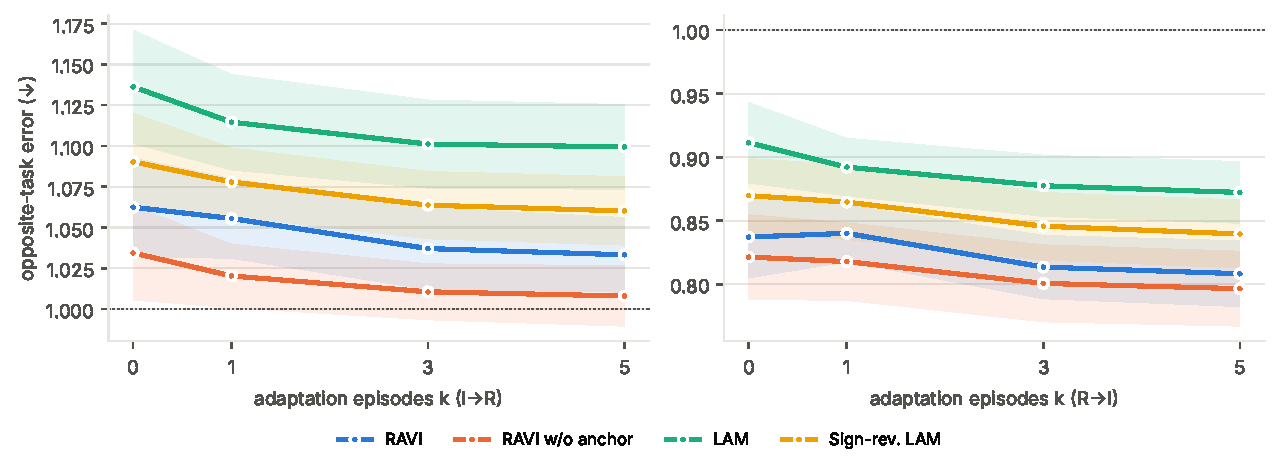
\includegraphics[width=\columnwidth]{figs/fig_fewshot_curves.pdf}
	\caption{Opposite-task error after fine-tuning the IDM on $k$ recordings (bands: s.d.).}
	\label{f:fewshot}
\end{figure}

When $\phi$ and $G_0$ are frozen and only the IDM is adapted, the two {\method} variants have the lowest opposite-task error of the models in Table~\ref{t:main} at every $k$ and in both directions (Fig.~\ref{f:fewshot}).
At $k=5$, {\method} without the anchor reaches 1.001 on I$\to$R and 0.804 on R$\to$I and the anchored model 1.029 and 0.815, against 1.076 and 0.868 for the plain LAM and 1.051 and 0.840 for sign reversal.
{\method} beats the LAM in 14 and 15 of 15 runs and in all 10 folds (Holm $p=0.009$ and $<0.001$), and the anchor costs some transfer, since the variant without it is better in 15 and 11 runs (Holm $p=0.30$ and $0.030$ over 10 folds).
The gap already exists at $k=0$, before any adaptation (1.058 and 0.846 against 1.109 and 0.904), and the Koopman ablations show that it comes from the Koopman forward model rather than from the shared drift: with $G_0=0$ the error is 1.025 and 0.813, no different from {\method} (Holm $p=1.0$ and $0.40$), the variant without reversal loss does not differ either (Holm $p=1.0$), {\method}-SR is slightly better for R$\to$I (Holm $p=0.048$), and fine-tuning $G_0$ together with the IDM gives 1.088 and 0.789.
For I$\to$R the error stays at or above the no-change level of 1.0 even after five recordings, so in that direction the advantage is a smaller deficit rather than useful prediction.

\subsection{Controlled Study with Known Drift} \label{s:toy}
To test the theory against ground truth, we simulate a point $p\in\R^2$ with $p_{t+1}=p_t+\Delta t\,(f(p_t)+u_t)$, $\Delta t=0.1$ and $u\in[-1,1]^2$, observed through a fixed random two-layer $\tanh$ lift to 32 dimensions, whose drift $f(p)=g-k\,w(p)\,(p-c)$ combines a pull $g=(0,-0.5)$ with a dissipative well of radius 1 around $c=(0,-1)$ ($w$ a smooth indicator, $k=3$).
The dynamics are first order, as Definition~\ref{d:trev} assumes, and each transition has a unique one-step undo $u^*=(p_t-p_{t+1})/\Delta t-f(p_{t+1})$, so a transition is reversible if $\|u^*\|_\infty\le2$, which fails only inside the well, for 21.7\% of transitions.
Idle steps ($u=0$, probability 0.15) anchor the models only outside the well, as on the robot.
Ten models ($d=8$, $m=2$, 4,000 steps, ten seeds) are evaluated on 6,000 fresh transitions (Table~\ref{t:toyd}), with a linear probe from latent to real actions fixing the gauge and undo actions executed in the simulator. Besides the robot-data models, they include {\method}-SR and the $G_0=0$ model without the anchor and a two-frame variant whose state $[o_t,\,o_t-o_{t-1}]$ carries velocity, with the velocity negated for swapped pairs.
Absorbed drift is the action size the probe reads on idle steps in the well relative to the mean, the AUROC compares irreversible with all or nearest-displacement reversible steps, and the return is the median distance to $p_t$ after undo in step lengths.
For reference, the feature change reaches an AUROC of 0.93 (0.61 at equal displacement) and the true drift magnitude 0.99, a random generator has a residual of 0.97, and the negated true action returns to 1.39 and 1.74 step lengths (reversible, irreversible), against best possible returns of 0 and 0.61.

\begin{table*}
	\centering
	\caption{Controlled study with known dissipative drift (mean $\pm$ 95\% CI half-width over 10 seeds). Returns in step lengths.}
	\label{t:toyd}
	\footnotesize
	\setlength{\tabcolsep}{2.5pt}
	\resizebox{\textwidth}{!}{%
	\begin{tabular}{lcccccccccc}
		\toprule
		& {\method} & w/o anchor & {\method}-SR & SR, no anchor & w/o reversal & $G_0=0$ & $G_0=0$, no anchor & Two-frame & LAM & Sign-rev. LAM \\
		\midrule
		Forward error $\downarrow$ & 0.30$\pm$0.01 & 0.02$\pm$0.00 & 0.34$\pm$0.04 & 0.01$\pm$0.00 & 0.14$\pm$0.01 & 0.42$\pm$0.04 & 0.02$\pm$0.00 & 0.27$\pm$0.01 & 0.02$\pm$0.01 & 0.02$\pm$0.00 \\
		IDM antisymmetry $\cos(\zb,-z)$ & 0.92$\pm$0.03 & 1.00$\pm$0.00 & 0.95$\pm$0.01 & 1.00$\pm$0.00 & 0.30$\pm$0.04 & 0.95$\pm$0.01 & 1.00$\pm$0.00 & 0.92$\pm$0.02 & 0.28$\pm$0.01 & 1.00$\pm$0.00 \\
		Absorbed drift, idle in well $\downarrow$ & 0.62$\pm$0.02 & 0.95$\pm$0.02 & 0.73$\pm$0.03 & 0.95$\pm$0.02 & 0.63$\pm$0.02 & 0.75$\pm$0.03 & 0.95$\pm$0.02 & 0.51$\pm$0.02 & 0.88$\pm$0.02 & 0.95$\pm$0.02 \\
		AUROC of $\kappa_t$, all steps & 0.69$\pm$0.03 & 0.92$\pm$0.01 & 0.80$\pm$0.02 & 0.92$\pm$0.00 & 0.60$\pm$0.01 & 0.84$\pm$0.01 & 0.92$\pm$0.00 & 0.75$\pm$0.02 & 0.75$\pm$0.03 & 0.75$\pm$0.07 \\
		AUROC of $\kappa_t$, equal displacement & 0.48$\pm$0.04 & 0.61$\pm$0.04 & 0.51$\pm$0.05 & 0.61$\pm$0.04 & 0.35$\pm$0.04 & 0.50$\pm$0.05 & 0.61$\pm$0.04 & 0.51$\pm$0.03 & 0.54$\pm$0.04 & 0.60$\pm$0.06 \\
		Drift residual $\varepsilon$ & 0.87$\pm$0.01 & 0.70$\pm$0.08 & 0.89$\pm$0.03 & 0.81$\pm$0.10 & 0.58$\pm$0.04 & -- & -- & 0.80$\pm$0.03 & -- & -- \\
		Return, reversible, closed form $\downarrow$ & 0.87$\pm$0.04 & 0.80$\pm$0.02 & 1.25$\pm$0.02 & 0.82$\pm$0.01 & 0.47$\pm$0.03 & 1.23$\pm$0.02 & 0.82$\pm$0.01 & 0.88$\pm$0.03 & 0.50$\pm$0.02 & 0.81$\pm$0.01 \\
		Return, reversible, planned $\downarrow$ & 0.92$\pm$0.06 & 0.77$\pm$0.02 & 0.72$\pm$0.04 & 0.79$\pm$0.02 & 0.50$\pm$0.06 & 0.89$\pm$0.05 & 0.80$\pm$0.02 & 0.70$\pm$0.07 & 0.42$\pm$0.03 & 0.78$\pm$0.02 \\
		Return, irreversible, planned $\downarrow$ & 1.08$\pm$0.03 & 1.35$\pm$0.03 & 1.33$\pm$0.02 & 1.35$\pm$0.03 & 1.02$\pm$0.05 & 1.36$\pm$0.02 & 1.35$\pm$0.03 & 1.13$\pm$0.03 & 1.08$\pm$0.02 & 1.36$\pm$0.02 \\
		\bottomrule
	\end{tabular}}
\end{table*}

Table~\ref{t:toyd} gives three findings that bear on our claims.
First, decoding under $-G_0$ reduces drift absorption only together with the anchor: on idle steps inside the well the probe reads 0.62 of the typical action size from {\method}, against 0.73 for {\method}-SR and 0.75 with $G_0=0$, with non-overlapping intervals, consistent with Proposition~\ref{p:signrev}. Without the anchor these three models are indistinguishable (0.95, like the sign-reversal LAM), the variant without reversal loss absorbs as little as {\method} (0.63), and the anchor costs most of the fit (forward error 0.30 against 0.01--0.02), so the anchor rather than the sign of the drift does most of the work.
Second, $\kappa_t$ detects irreversible steps through their motion rather than their irreversibility: its AUROC of 0.60--0.92 against all reversible steps falls to 0.35--0.61 for every model at equal displacement, while the true drift magnitude stays at 0.99, and the state-dependent scores do not help, since $\rho_t$ is mostly below chance (0.21--0.58) and $\varepsilon_t$ is inconsistent across variants (0.39--0.82).
Third, the drift correction of the undo action matters where the drift can be cancelled: on reversible steps the closed-form undo $-z-2c$ returns the point to within 0.87 step lengths, against 1.25 for $-z$ in {\method}-SR, 1.23 with $G_0=0$ and 1.39 for the negated true action, but without the anchor all drift variants reach 0.80--0.82, the plain LAM (0.50) and the variant without reversal loss (0.47) do better, and after planning anchored {\method} is worst (0.92 against 0.42 for the LAM); on irreversible steps every model stays above 1.0 against a best possible 0.61.
Removing the reversal loss lowers the IDM antisymmetry from 0.92 to 0.30, as Remark~\ref{r:reduce} implies, and residuals of 0.58--0.89, below the random 0.97, show that here the actions cancel part of the drift. The two-frame variant, whose state carries velocity, fits like anchored {\method} (0.27), absorbs the least drift (0.51) and plans better undo actions (0.70), but its score is still at chance at equal displacement (0.51).

% =====================================================================
\section{Discussion and Limitations} \label{s:discussion}

\paragraph{What the evidence supports.}
The cross-validated results support three claims that hold in every run: Koopman models trained with a reversal loss avoid the divergence and the below-chance detection of an MLP sign-reversal model, the condition number of the learned step separates post-release windows from grasped carrying above chance, and the Koopman variants transfer best to the opposite task when only the IDM is adapted. Holm-corrected fold-level tests over ten folds support the transfer gain over both LAM baselines, the stability gain over the model without reversal loss, and the gains over sign reversal in end distance and transfer (I$\to$R) and in detection (R$\to$I).
In the controlled study, decoding swapped pairs under $-G_0$ with an anchor absorbs less passive motion than under $+G_0$, and the drift correction improves the closed-form undo action, which is consistent with Propositions~\ref{p:undo} and~\ref{p:signrev}.

\paragraph{What it does not.}
On the robot data, the gains cannot be credited to the drift-aware loss: decoding swapped pairs under $+G_0$ makes reverse rollouts at least as stable and leaves detection, transfer and absorption unchanged, stability comes from the reversal loss in Koopman form, and transfer comes from the Koopman forward model, since it persists with $G_0=0$.
Because the drop is brief and triggered by the agent, a sign-reversal model can probably attribute it to the release at little cost.
{\method} is not more stable than a plain LAM, whose reverse actions improve more on its own null and align better with the real ones, and its detection mostly reflects motion: proprioceptive cues beat every learned score. The anchor raises detection but costs transfer, probably because idle steps rarely coincide with strong drift in this task.
The drift residual near 0.99 equals that of a random drift, so $\zundo$ reduces to $-z$; state-specific undo leaves the same absolute error after drops as after carrying; and insertion-to-removal transfer stays at the no-change level.
In the controlled study, $\kappa_t$ again detects only larger motion, $\rho_t$ and $\varepsilon_t$ do not detect irreversibility, and a plain LAM undoes reversible steps best.

\paragraph{Lessons for latent action models.}
Three lessons carry over to other latent action models. First, a reversal constraint is only as good as the forward model it is imposed on: the same sign-reversal idea diverges with an MLP, even under zero actions, but stays stable in Koopman form, so rollouts must be compared with each model's own null before reverse actions are credited.
Second, a reversibility score must be tested against negatives of equal motion and against proprioceptive cues, because a score can separate releases from carrying simply by detecting the release motion, as $\kappa_t$ does on the robot and in the controlled study.
Third, a drift residual needs a reference value, such as Remark~\ref{r:eps} or a random drift of equal norm, before it can be read as evidence about the physics; on our data the two are indistinguishable.

\paragraph{Scope.}
We evaluate one task, one camera view for the dynamics and a frozen encoder, with three seeds per fold over five folds and one seed per fold over ten.
The latent state is computed from a single frame and its dynamics are first order, so Definition~\ref{d:trev} reverses the learned dynamics rather than the mechanics, and momentum is not represented.
The drop is triggered by the agent and completes within one 0.5\,s step in an otherwise static scene, which a constant drift generator applied at every state models only coarsely.
The anchor uses proprioceptive joint speed, so the anchored model is not trained from video alone, and the strip condition of the theory, verified here for every 0.5\,s step, must be checked again for longer horizons.

\paragraph{Outlook: deformable objects.}
Folding clothes would be an informative next benchmark, because a single task contains both regimes~\cite{lin2020softgym,lin2021vcd}.
Slow folding motions are close to reversible, whereas draping and settling after release dissipate energy, so their Koopman modes satisfy $|\lambda|<1$, and cloth is usually unfolded by flinging or regrasping rather than by reversing the fold~\cite{ha2021flingbot,avigal2022speedfolding}.
Koopman models already control soft robots~\cite{bruder2019soft}, and because settling continues after the gripper lets go, cloth offers passive motion without agent action, which the toaster task lacks. We expect state-dependent scores such as $\rho_t$ and $\varepsilon_t$ to separate fold and settle phases, and state-specific undo to quantify how much of a fold can be undone in one step.

% =====================================================================
\section{Conclusion} \label{s:conclusion}

Recovering reverse actions from video depends on telling the agent's effect apart from the scene's own motion, and {\method} expresses this separation with a Koopman operator whose drift generator is distinct from its action generators.
Trained only on forward footage, it delivers an exact backward step in the lifted space, the time-reversal action of the first-order latent dynamics, the undo action and a reversibility score, and we proved when each is exact, why sign reversal in Koopman form forces zero drift, why the split between agent and drift must be anchored, and why a drift residual near 1 is expected when actions and drift are unrelated.
On real bimanual robot data over five folds and three seeds, the reverse rollouts of {\method} remained stable where an MLP sign-reversal model diverged, releases were detected above chance and transfer to the opposite task was the best among the compared models, gains that the ablations credit to the reversal loss and the Koopman form rather than to the reversed drift.
In a controlled study with known drift, decoding under the reversed drift absorbed less passive motion when the split was anchored and the drift correction improved the closed-form undo action, consistent with the theory, while the reversibility score tracked motion rather than irreversibility.
Multi-step undo, state-dependent reversibility scores, velocity-aware latent states and deformable objects are the next steps.

\bibliographystyle{IEEEtran}
\bibliography{ravi}

\ack{To be added after review.}

\authorbio{photo_emaase}{Patrick Mokodir Emaase}{Department of Computer Science and Engineering, Seoul National University, Seoul, Korea (emaase@bi.snu.ac.kr).}
\authorbio{photo_choi}{Choi Suhyung}{AI Institute, Seoul National University, Seoul, Korea (shchoi@bi.snu.ac.kr).}
\authorbio{photo_zhang}{Byoung Tak Zhang}{Department of Computer Science and Engineering, Seoul National University, Seoul, Korea (btzhang@snu.ac.kr).}

\end{document}
